% Dies ist die Hauptdatei, von der aus das Gesamtdokument erzeugt wird.  Diese
% Datei sollten Sie zunächst umbenennen, damit sie keinen generischen Namen
% hat!  Dann wird sie mit LuaLaTeX kompiliert.

% In der Datei defs.tex werden alle globalen LaTeX-spezifischen Einstellungen
% vorgenommen
% Jede LaTeX-Datei beginnt mit der Dokumentenklasse.  Für diese Vorlage wurde
% die Klasse "scrreprt" von KOMA-Script gewählt, die in etwa der
% Standardklasse "report" entspricht, allerdings wesentlich mehr Möglichkeiten
% bietet und im gewissen "moderner" ist.  Eine sehr ausführliche Dokumentation
% zu KOMA-Script findet man unter der folgenden Adresse:
% http://mirrors.ctan.org/macros/latex/contrib/koma-script/doc/scrguide.pdf
\documentclass[
% die Schriftgröße - sollten Sie nicht ändern
    fontsize=12pt,
% das Papierformat, also DIN A4
    paper=A4,
% Literaturverzeichnis ins Inhaltsverzeichnis
    bibliography=totoc,
% andere Verzeichnisse ebenfalls ins Inhaltsverzeichnis
    listof=totoc,
% abgesetzte Formeln linksbündig
    fleqn,
% für die Satzspiegelkonstruktion - siehe KOMA-Doku
    DIV=12,
% Bindekorrektur (linker Rand) - evtl. anpassen
    BCOR=1mm,
% die im Text verwendeten Sprachen (u.a. für das Paket babel); die
% letztgenannte (!) Sprache ist die Standardsprache; "n"german steht für die
% neue Rechtschreibung
    english,
% weil (s.u.) das Paket geometr verwendet wird
    usegeometry,
% wie Absätze gesetzt werden: ohne Einzug, halbe Zeile Abstand
    parskip=half-
]{scrreprt}

\usepackage{subcaption}
% Beschriftungen für Tabellen kommen linksbündig über die Tabelle
\KOMAoption{captions}{tableheading}
\setcaptionalignment[figure]{c}
\setcaptionalignment[table]{l}

% wird für die Titelseite benötigt
\usepackage{geometry}

% Standardpaket für Lokalisation, siehe Option "ngerman" oben
\usepackage{babel}
% Laden von optimierten Trennmustern
\babelprovide[hyphenrules=ngerman-x-latest]{ngerman}

% Standardpaket für mathematische Zusatzfunktionen; wenn Sie keine
% mathematischen Formeln brauchen, können Sie diese Zeile löschen
\usepackage{amsmath}

% die Hauptschrift Libertinus
\usepackage{libertinus-otf}
% die "Schreibmaschinenschrift" Anonymous Pro, angepasst
\usepackage{AnonymousPro}
\setmonofont{AnonymousPro}[Scale=MatchLowercase,FakeStretch=0.85]

% etwas größerer Zeilenabstand als im Buchsatz
\linespread{1.1}

% Paket für Feinkorrekturen an der Typographie, das für ein ausgewogeneres
% Schriftbild sorgt
\usepackage{microtype}

% Paket für kontextsensitive Anführungszeichen
\usepackage{csquotes}
% Shortcut, damit aus dem eigentlich falschen Zeichen " richtige
% Anführungszeichen je nach Sprache werden
\MakeOuterQuote{"}

% Paket, das den Befehl \includegraphics ermöglicht
\usepackage{graphicx}

% komfortablere Aufzählungen als in Standard-LaTeX; ein Beispiel findet man in
% chap3.tex
\usepackage{enumitem}

% Paket für mehr als die üblichen Standardfarben
\usepackage[dvipsnames]{xcolor}
% Definition der "Hausfarben" der HAW
\definecolor{haw}{HTML}{003CA0}
\definecolor{haw2}{HTML}{0096D2}
\definecolor{haw3}{HTML}{A0BEDC}

% typographisch anspruchsvolle Tabellen; siehe chap3.tex
\usepackage{booktabs}

% zum Erstellen des Literaturverzeichnisses; der gängige Stil APA ist hier
% bereits eingestellt
\usepackage[style=apa]{biblatex}
% eine Beispieldatei für ein Literaturverzeichnis
\addbibresource{demo.bib}

% für die Erzeugung der Grafiken in chap3.tex; wenn Sie PGF/TikZ nicht
% verwenden wollen, können Sie diese Zeilen entfernen
\usepackage{tikz}
% Zusatzbibliotheken für TikZ, die in den genannten Beispielen verwendet
% werden
\usetikzlibrary{calc,intersections,angles,3d}

% für die Erzeugung des Codeblocks in chap3.tex; wenn in Ihrer Arbeit keine
% Codeblöcke vorkommen, können Sie diese Zeilen entfernen
\usepackage{listings}
% Anpassung des Erscheinungsbildes des Codeblocks; mehr dazu in der
% Dokumentation des Pakets "listings"
\lstdefinestyle{mystyle}{
    backgroundcolor=\color{gray!20},
    keywordstyle=\color{haw2},
    numberstyle=\footnotesize\color{haw},
    basicstyle=\ttfamily\small,
    captionpos=t,
    frame=single,
    framerule=0pt,
    keepspaces=true,
    numbers=left,
    numbersep=6pt,
    belowcaptionskip=1em,
    aboveskip=\bigskipamount,
}
\lstset{style=mystyle}
% damit es "Codeblock" und nicht "Listing" heißt
\renewcommand{\lstlistingname}{Codeblock}

% für die Verlinkung innerhalb des PDF-Dokuments, für PDF-Lesezeichen und
% PDF-Metadaten; dieses Paket sollte üblicherweise immer als letztes geladen
% werden
\usepackage[colorlinks=true,allcolors=haw,hyperfootnotes=false,pageanchor=true,linktoc=all]{hyperref}

% für die Druckversion können Sie die obige Zeile durch die folgende ersetzen,
% damit Links nicht blau dargestellt werden:
% \usepackage[draft]{hyperref}

% Metadaten des PDF-Dokumentes; setzen Sie hier Ihren eigenen Namen sowie den
% Titel Ihrer Arbeit ein
\hypersetup{pdfauthor={Prof. Dr. Edmund Weitz}}
\hypersetup{pdftitle={Handreichung zur Formatierung von Bachelorarbeiten}}


% Wenn das Kommentarzeichen entfernt wird, kann man mit einem Befehl wie
%
% \includeonly{chap2,chap3}
%
% erreichen, dass nur ausgewählte Dateien kompiliert werden.  Das ist für die
% Arbeit an umfangreichen Dokumenten hilfreich, weil es Zeit spart.  Für das
% Erstellen des fertigen Dokuments muss der Befehl natürlich wieder
% auskommentiert werden, damit alle Referenzen aktuell sind und die
% Seitenzahlen stimmen.

% Hier beginnt das eigentliche Dokument.  Sie können weitere Dateien
% hinzufügen und natürlich auch vorhandene weglassen.  Die vorhandene
% Dateistruktur ist lediglich als Beispiel gedacht.
\begin{document}
% In dieser Umgebung wird die Titelseite separat vom restlichen Text gesetzt
\begin{titlepage}
  % andere Seitenränder als im Rest der Arbeit
  \newgeometry{lmargin=2cm,tmargin=7mm,rmargin=5mm,bmargin=1cm}
  % die "Hausfarbe" der HAW; diese und die folgenden Einstellungen sind lokal
  % und gelten nur innerhalb der Umgebung "titlepage"
  \color{haw}
  % Blocksatz für die Titelseite deaktivieren
  \raggedright
  % Logo rechtsbündig setzen
  \hfill
\includegraphics[width=7cm]{images/HAW_Marke_RGB_300dpi}\\

  % vertikaler Abstand
  \vspace{5cm}

  % Wahl der "Hausschrift" Open Sans der HAW, die als Schrift auf Ihrem
  % Rechner installiert sein muss
  \setmainfont{Open Sans}
  % etwas kleiner als üblich
  \small
  % fett und in Majuskeln
  \textbf{BACHELORARBEIT}

  % vertikaler Abstand
  \vspace{8mm}

  % der Titel der Arbeit als "Seite in der Seite"; natürlich müssen Sie hier
  % Ihren Titel eintragen
  \begin{minipage}{0.8\linewidth}
    % Wahle der zweiten "Hausschrift" der HAW, die ebenfalls auf Ihrem Rechner
    % bereits vorhanden sein muss
    \setmainfont{Martel Heavy}
    % ziemlich große Schrift
    \LARGE
    % [1mm] steht jeweils für einen etwas größeren Durchschuss

    Detecting Geometric Primitives\\[1mm]
    in Depth Data from the\\[1mm]
    Google ARCore Depth API\\[1mm]
    \,\rule{11mm}{1.2mm}
  \end{minipage}

  % vertikaler Abstand, überraschenderweise
  \vspace{1cm}

  % hier korrektes Datum und Ihren Namen eingeben
  vorgelegt am 01.\ Februar 1900\\
  Hugo Protsch

  % letzter vertikaler Abstand für heute
  \vspace{5cm}

  % noch eine "Seite in der Seite", etwas nach rechts geschoben
  \hspace*{37mm}
  \begin{minipage}{0.5\linewidth}
    % Namen und Titel der beiden Prüfer eintragen
    \begin{tabular}{@{}ll}
      Erstprüferin: & Prof. Dr. Philipp Jenke\\[-.3mm]
      Zweitprüfer: & Prof. Dr. Olaf Zukunft\\
    \end{tabular}\\

    % noch ein horizontaler Strich
    \,\rule{9mm}{1mm}\\[1.5mm]

    \textbf{HOCHSCHULE FÜR ANGEWANDTE}\\
    \textbf{WISSENSCHAFTEN HAMBURG}\\
    Department Informatik\\
    Berliner Tor 7\\
    20099 Hamburg
  \end{minipage}
\end{titlepage}
% setzt die Geometrie wieder auf die Standardwerte zurück
\restoregeometry

% für die Seite mit dem Abstract keine Seitenzahl ausgeben
\thispagestyle{empty}



\thispagestyle{empty}
\clearpage

% In der Titelei werden römische Ziffern für die Seitenzahlen verwendet;
% gleichzeitig wird durch diesen Befehl die aktuelle Seitenzahl auf eins
% gesetzt
\pagenumbering{Roman}

% Inhaltsverzeichnis
\tableofcontents

% Abbildungsverzeichnis, kann evtl. weggelassen werden
\listoffigures

% Tabellenverzeichnis, kann evtl. weggelassen werden
%\listoftables

% weitere Verzeichnisse (z.B. Codeblöcke) sind theoretisch möglich

% neue Seite, vorsichtshalber
\clearpage
% ab jetzt arabische Ziffern und wieder auf eins setzen
\pagenumbering{arabic}

\section*{Abstract}
This thesis aims to detect geometric primitives, such as planes, spheres, and cylinders,
within three-dimensional data obtained from mobile devices.
The primary objective is to generate a 3D model of an interior space, which encompasses furniture and other objects.
An additional (optional) objective may involve the detection and categorization of these objects.
Depth information from the Google ARCore SDK, which does not require specialized depth-sensing hardware, will be used.



\paragraph*{Keywords}
Augmented Reality, Surface Reconstruction, Point Clouds, Depth Maps, Primitive Extraction, Object representation, Object Detection, Mobile Applications

\section*{Summary}

The aim of this thesis is to provide an end-to-end implementation of a system
that can detect primitives on a mobile device using data from the Google ARCore Depth API
and render a mesh of the detected primitives overlaid onto the camera feed.

\chapter{Introduction}

\section{Research Aims}
%Object detection and classification are fundamental problems of both Augmented Reality (AR) and computer vision.

%The following questions are under consideration.
%\begin{enumerate}
%    \item What is the nature of the objects to be detected? Should the items be geometric primitives themselves, or should more complex items be approximated using geometric primitives?
%    \item How should the selection of objects for tracking be determined? Should the algorithm autonomously identify the most suitable approximation, or should the process be guided by user interaction, such as selecting an object on the screen to initiate detection?
%    \item Should multiple objects be detected at the same time?
%    \item Should the objects be tracked? If yes, under which conditions? Should tracking occur:
%    \begin{enumerate}
%        \item while the device is in motion,
%        \item while the object itself is in motion, or
%        \item under a combination of both conditions?
%    \end{enumerate}
%    \item Should the detection be reevaluated as new data arrives?
%    \item Which assumptions can be made about the environment?
%\end{enumerate}
%

\section{Background}

\subsection{Augmented Reality, Virtual Realtiy and Mixed Reality}

\subsection{Trends in the industry}

\paragraph{Google Glasses}

\paragraph{Meta Quest 3}

\paragraph{Apple Vision Pro}

\section{Related Work}

\chapter{Primitive Detection Algorithms}\label{ch:primitive-detection-algorithms}

\begin{figure}[ht!]
    \centering
    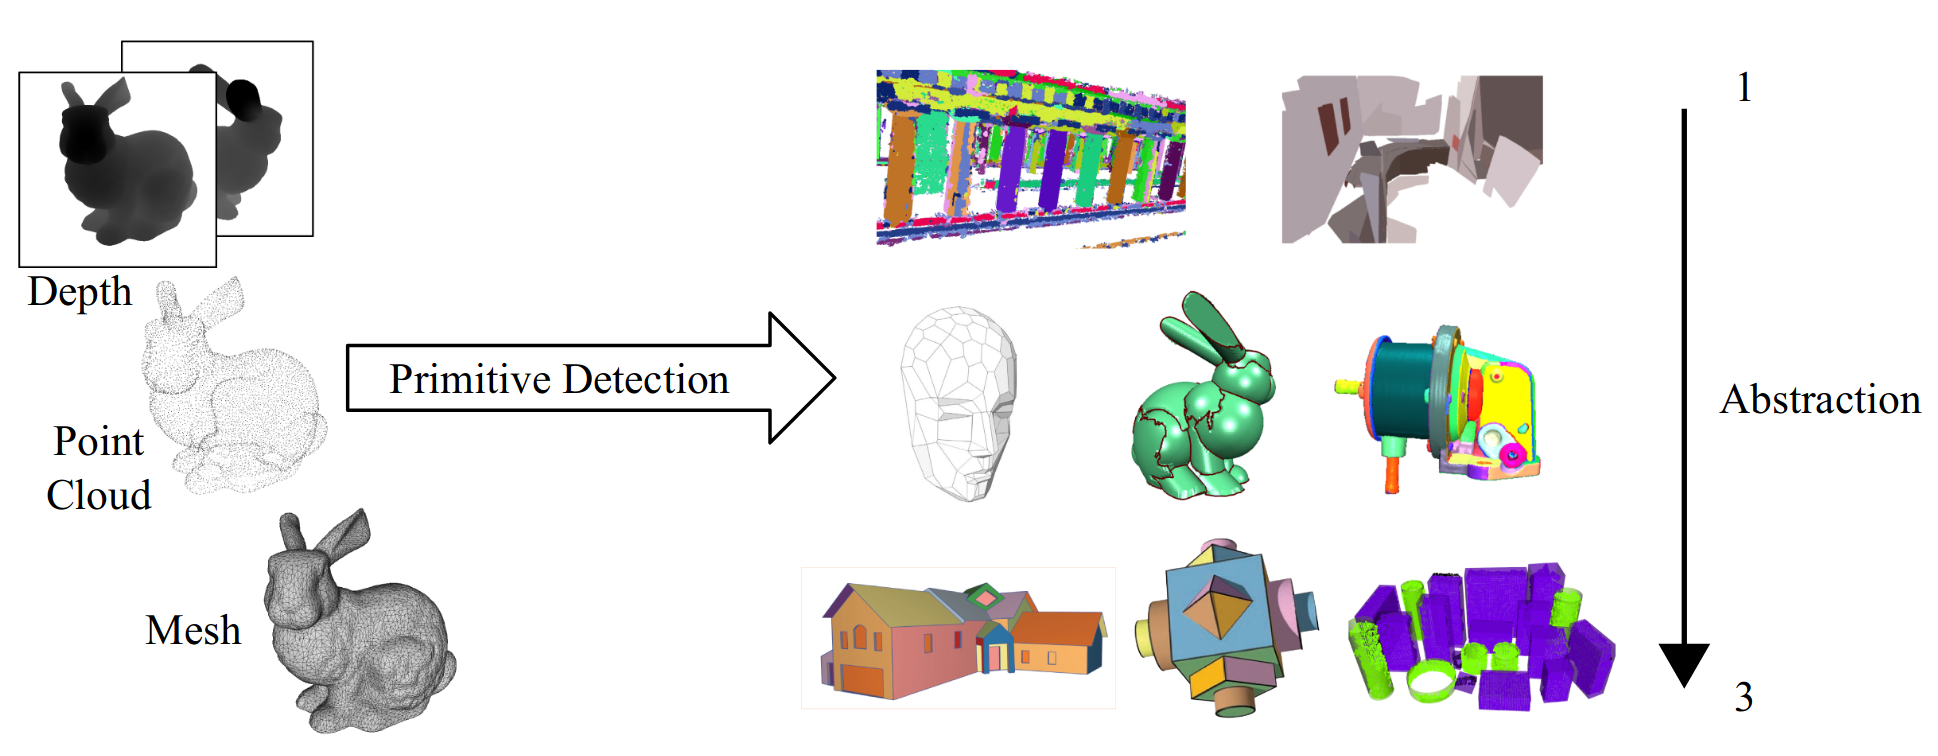
\includegraphics[width=\linewidth]{images/primitive_detection}
    \caption{Process of detecting primitives \cite{kaiser_survey_2019}}
    \label{fig:primitive_detection}
\end{figure}
Primitive detection is a well-established area in computer vision that aims to detect simple geometric shapes
like planes, spheres or cylinders in given input data.
These methods are model-fitting algorithms that identify the most likely model that fits (a subset of) the input data.
The result of these algorithms is a set of parameters that describe the detected shape.
These shapes are an abstraction of the input data, offering a simplified compact representation of the data,
allowing for higher performance and the ability to perform higher-level tasks such as object recognition or scene reconstruction.
The input data representation varies by algorithm, with the most common types being:
\begin{itemize}
    \item \textbf{Point Clouds:} A set of 3D points in space representing the sampled surface of the real-world
    \item \textbf{Depth Images:} A 2D image where each pixel represents the distance to the camera, typically obtained from depth sensors
    \item \textbf{Image Sequences:} A sequence of 2D images from different viewpoints that are typically first convert to a point cloud or depth image for further processing, further discussed in section~\ref{sec:technical-background-depth-from-motion}
    \item \textbf{Meshes:} A polygonal representation of surfaces, consisting of vertices, edges, and faces, typically generated from surface reconstruction algorithms.
    Not further considered in this thesis.
    For an explanation of meshes, see section~\ref{subsec:polygon-meshes}.~\cite{kaiser_survey_2019}
\end{itemize}

This chapter provides an overview of the most common primitive detection algorithms by categorizing them based on their underlying methodology.
The chapter then compares the two most widely used base methodologies,
the Hough Transform and the Random Sample Consensus (RANSAC) algorithm.


\section{Categorization}
\citeauthor{kaiser_survey_2019}~\cite{kaiser_survey_2019} reviewed over 70 detection algorithms, evaluating them based on their input/output data types,
underlying methodology, supported primitive types, context of application and provides a rating for multiple criteria.
The authors categorize the underlying methodology of the algorithms into three categories:
\begin{itemize}
    \item \textbf{Stochastic:} algorithms that use random sampling to detect primitives, such as RANSAC
    \item \textbf{Parameter Space:} algorithms that use a parameter space to detect primitives, such as the Hough Transform
    \item \textbf{Other techniques}, for example primitive-driven region growing
\end{itemize}

The following sections provide an overview of the most common algorithms in each category.

\subsection{RANSAC (Stochastic)}
The Random Sample Consensus (RANSAC) algorithm is a widely used stochastic model parameter estimation
algorithm first introduced in~\citeyear{fischler_random_1981}
by~\citeauthor{fischler_random_1981}~\cite{fischler_random_1981}.
"The basic principle of the algorithm is to try many possible randomized models that could fit
the data and evaluate how good this model is in order to find a consensus,
i.e.\ an agreement of most of the data samples."~\parencite{kaiser_survey_2019}

For a given shape that requires $n$ points to be defined, RANSAC follows the following steps to detect the shape
in a set of data points $P$~\parencite{fischler_random_1981}:
\begin{enumerate}
    \item Randomly select a subset $S1$ of $n$ data points from $P$
    \item Fit the model $M1$ to the selected points
    \item Determine the subset of inliers $S1^*$ of $P$ that fit the model $M1$ within a predefined tolerance, this is called the consensus set
    \item If size of the consensus set $|S1^*|$ is greater than a predefined threshold $t$, re-fit the model to $S1^*$, resulting in new model $M1^*$
    \item If size of the consensus set $|S1^*|$ is smaller than a predefined threshold $t$, repeat until a model with a consensus set of size $t$ is found or a predefined number of iterations is reached
\end{enumerate}

The algorithm has 3 main parameters that need to be set:
\begin{itemize}
    \item \textbf{Error tolernace:} the distance between a data point and the model under which the data point is considered an inlier
    \item \textbf{Threshold $t$:} the number of inliers required to consider a model valid
    \item \textbf{Number of iterations:} the number of times the algorithm will try to find a model with a consensus set of size $t$
\end{itemize}

\subsection{Hough Transform (Parameter Space)}
The Hough transform (HT) introduced in~\citeyear{hough_method_1962}~\parencite{hough_method_1962}
is an algorithm that was originally designed to detect lines in images,
but has since been generalized to detect more complex shapes like circles~\cite{ballard_generalizing_1981} and 3D shapes~\cite{woodford_demisting_2014}.

The HT works by creating a voting space based on parameters where similar shapes overlap\cite{kaiser_survey_2019}.
The following explanation of the HT is based on~\cite{shree_k_nayar_first_2021}.
Figure~\ref{fig:hough-transform} illustrates the concept of the Hough Transform for detecting lines.
On the left, the image space is shown, where 4 points are located on a line.
The right side shows the parameter space, where the axes represent the parameters of the line equation
\begin{equation}
    y = mx + c
\end{equation}
Each point in image space creates a line in parameter space, as there are an infinite number of lines that pass through a point.
All points on the line represent a valid parameterizations of the line.
When all points are plotted in parameter space, local maxima represent possible lines that fit the input data.
\begin{figure}[ht!]
    \centering
    \begin{subfigure}[t]{0.45\textwidth} % Adjusted from 0.4 to 0.45
        \centering
        \begin{tikzpicture}

            % Axes
            \draw[->] (0,0) -- (4,0) node[right] {$x$};
            \draw[->] (0,0) -- (0,4) node[above] {$y$};

            % Line
            \draw[dashed] (0.5,1) -- (4.5,4);

            % Points on the line y = 0.75x + 0.625
            \foreach \x in {1, 2, 3, 4} {
                \pgfmathsetmacro\y{0.75*\x + 0.625}
                \filldraw (\x,\y) circle (2pt);
            }

%        % Label for a point
%        \draw[->] (2,2.125) -- (2.5,2.5) node[above] {$(x_i, y_i)$};

            % Equation
            \node at (2.5,-0.5) {$y_i = mx_i + c$};

            % Title
%            \node at (2.5,5.5) {\textbf{Image Space}};


        \end{tikzpicture}
        %    source: szeliski_computer_nodate
        \caption{Image Space}
        \label{fig:ht-1}
    \end{subfigure}%
    \hspace{0.05\textwidth} % Added space between subfigures
    \begin{subfigure}[t]{0.45\textwidth} % Adjusted from 0.4 to 0.45
        \centering
        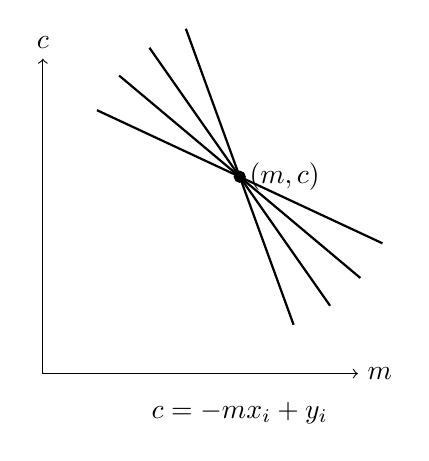
\begin{tikzpicture}
            % Draw axes
            \draw[->] (0,0) -- (4,0) node[right] {$m$};
            \draw[->] (0,0) -- (0,4) node[above] {$c$};
            % Define the point (m, c)
            \coordinate (mc) at (2.5,2.5);
            % Draw the point (m, c)
            \filldraw (mc) circle (2pt) node[right] {$(m,c)$};
            % Draw lines radiating from the point (m, c)
            \foreach \angle in {0, 15, 30, 45} {
                \draw[thick] (mc) -- ++(\angle-70:2);
                \draw[thick] (mc) -- ++(\angle-70+180:2);
            }
            % Add the equation below the graph
            \node at (2.5,-0.5) {$c = -mx_i + y_i$};
        \end{tikzpicture}

        \caption{Parameter Space}
    \end{subfigure}%
    \caption{Concept of Hough Transform illlustrated for the usage of detecting lines. Based on \cite{shree_k_nayar_first_2021}.}
    \label{fig:hough-transform}
\end{figure}

The Hough Transform is implemented by discretizing the parameter space into uniform sections
using a two-dimensional array to store the votes for each parameter, called the accumulator~\parencite{duda_use_1972}.
Each data point contributes votes to the shapes it aligns with, indicating the likelihood of a specific shape being present in the input data.
By accumulating these votes, the parameters corresponding to the shape with the highest number of votes can be identified.
After all data points have voted, the parameters with the highest votes reveal the shape that most accurately fits the input data.

A problem that arises when using the Hough Transform using the standard parameterization of a line $y = mx + c$
is that the slope $m$ can be infinite for vertical lines, which would require the parameter space to be infinite.
To solve this problem, a parameterization using the angle from the x-axis $\theta$ and the distance from the origin $\rho$ is used:
\begin{equation}
    x \sin \theta + y \cos \theta = \rho = 0
\end{equation}
\begin{figure}[ht!]
    \centering
    \begin{subfigure}[t]{0.45\textwidth}
        \centering
        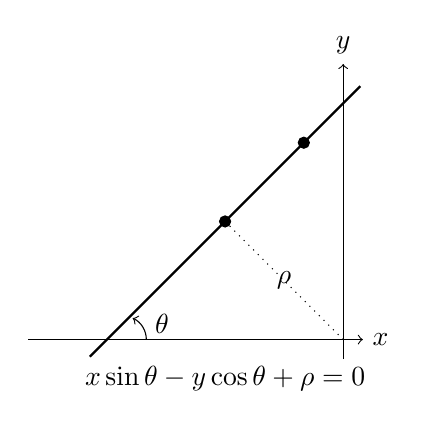
\begin{tikzpicture}
            % Draw axes
            \draw[->] (-4,0) -- (0.25,0) node[right] {$x$};
            \draw[->] (0,-0.25) -- (0,3.5) node[above] {$y$};

            % Draw the line
            \draw[thick, shorten <=0.4cm, shorten >=0.4cm] (-3.5,-0.5) -- (0.5,3.5);

            % Draw the perpendicular distance
            \draw[dotted] (0,0) -- (-1.5,1.5);

            % Draw the dots
            \filldraw (-1.5,1.5) circle (2pt);
            \filldraw (-0.5,2.5) circle (2pt);

            % Mark the angle theta
            \draw[->] (-2.5,0) arc[start angle=0,end angle=65,radius=0.3];
            \node at (-2.3,0.2) {$\theta$};


            % Label rho
            \node at (-0.75,0.75) {$\rho$};


            % Label the equation
            \node at (-1.5,-0.5) {$x \sin \theta - y \cos \theta + \rho = 0$};
        \end{tikzpicture}


        %    source: szeliski_computer_nodate
        \caption{Image Space}
        \label{fig:ht-polar-1}
    \end{subfigure}%
    \hspace{0.05\textwidth} % Added space between subfigures
    \begin{subfigure}[t]{0.45\textwidth} % Adjusted from 0.4 to 0.45
        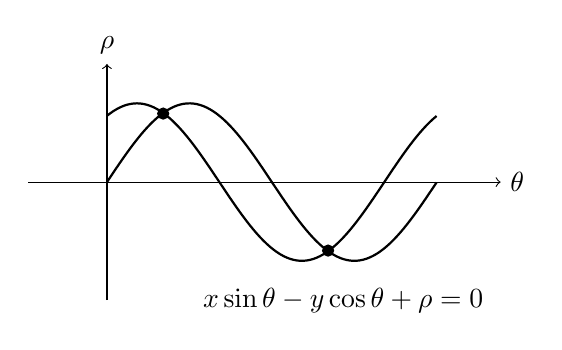
\begin{tikzpicture}
            % Draw axes
            \draw[->] (-1,0) -- (5,0) node[right] {$\theta$};
            \draw[->] (0,-1.5) -- (0,1.5) node[above] {$\rho$};

            % Draw the sinusoidal curve
            \draw[thick, domain=0:0.6666*6.28, samples=100] plot (\x, {sin(1.5*\x r)});
            \draw[thick, domain=0:0.6666*6.28, samples=100] plot (\x, {sin((1.5*\x + 1) r)});

            \filldraw (0.71386, 0.87) circle (2pt);
            \filldraw (2.80826, -0.87) circle (2pt);

            % Label the equation
            \node at (3,-1.5) {$x \sin \theta - y \cos \theta + \rho = 0$};
        \end{tikzpicture}

        \caption{Parameter Space}
        \label{fig:ht-polar-2}
    \end{subfigure}%
    \caption{Hough Transform using polar coordinates. Based on \cite{shree_k_nayar_first_2021}.}
    \label{fig:hough-transform-polar}
\end{figure}
This parameterization allows for the representation of all lines, including ones that are vertical,
as the angle $\theta$ can be any value between $0$ and $\pi$; the distance $\rho$ between $0$ and the size of the image space.
This also decreases the size of the accumulator array.
To detect lines using this parameterization, the same voting process as described above is used.


\subsection{Primitive-driven Region Growing}
TODO


\section{Choosing an algorithm: Hough Transform vs RANSAC}\label{sec:choosing-an-algorithm}

\cite{kaiser_survey_2019} lists over 70 detection algorithms, many of which are specialized for specific application contexts
like indoor scenes, outdoor scenes, urban buildings or individual objects.
As this thesis aims to develop a general end to end implementation for detecting and rendering primitives in AR,
algorithms that are widely used and applicable to a wide range of applications will be considered.
Both the Hough Transform and the Random Sample Consensus (RANSAC) algorithm stand out as the
most widely used methodologies in the field of primitive detection~\parencite{schnabel_efficient_2007}.
This section provides a comparison of these two methodologies and a decision on which algorithm to use for the implementation.

In general, the performance of both algorithms varies based on the context of the application.
With optimizations, both algorithms are suitable for a wide range of applications, but
the Hough Transform is more computationally expensive than RANSAC~\parencite{kaiser_survey_2019}.
\cite{tarsha-kurdi_hough-transform_2007} found that its processing time is negligible in comparison to the Hough Transform.
RANSAC is also more robust to noise and outliers~\parencite{kaiser_survey_2019}.
It is also simpler and therefore easier to extend and adapt to different contexts~\parencite{tarsha-kurdi_hough-transform_2007, kaiser_survey_2019}.
The main drawback of RANSAC is that results are not repeatable, as the algorithm is based on random sampling~\parencite{kaiser_survey_2019}.


For a concrete example,~\cite{tarsha-kurdi_hough-transform_2007} analyzed the application of detecting building
roofs as planes in 3D Lidar scans of cityscapes, and found that by default both RANSAC and Hough-Transform yield similar,
insufficient results for their use-case.
“That can be explained by the use of a pure mathematical principle,
without taking into account the particularity of the building Lidar data. […] That is why
[they] may detect a set of points which represents several roof planes or which belongs to several planes.”
They also had difficulties to determine the parameters of Hough Transform,
as the optimal values vary based on the characteristics of the point cloud.
Motivated by RANSACS rapidity they investigated extending the RANSAC algorithm and with their improvements
found that it produces satisfying results.

In the end, both the Hough Transform and RANSAC are suitable algorithms for detecting primitives.
However, the Hough Transform is more computationally expensive, harder to tune for specific contexts and less robust to noise and outliers.
RANSAC also has a publicly available reference implementation in C\texttt{++} by~\parencite{schnabel_efficient_2007},
which is e.g.\ used in the open source tool CloudCompare~\parencite{daniel_girardeau-montaut_cloudcompare_nodate} and can therefore be
easily tested on ones own pointclouds without the need to write custom code, useful for evaluation, as can later be seen in chapter~\ref{ch:evaluation}.

Due to these reasons, the Random Sample Consensus (RANSAC) algorithm will be used for the implementation of the primitive detection in this thesis.

\chapter{Implementation Context}

\section{Requirements and Constraints}

\paragraph{Accuracy might vary based on many variables}

\begin{enumerate}
    \item Object texture
    \item Distance
    \item Lighting conditions
\end{enumerate}

\paragraph{Near-real-time (once every 10s or so)}

\paragraph{Limited processing power (smartphone)}


\section{Potential pitfalls}
As the development device, Google Pixel 7, does not have a depth sensor,
the Depth API will exclusively utilize depth-from-motion techniques to derive depth information from camera images.
However, it is important to note that camera-based depth-from-motion has limitations
when it comes to detecting depth in objects with minimal texture, such as walls.
This drawback could potentially present challenges.
For instance, if the objective were to recognize objects like boxes or spheres that lack texture,
the accuracy of depth information obtained from the Depth API may not be sufficient for accurate recognition. \parencite{google_llc_arcore_doc}

\section{Hard- and Softwarestack}

The mobile application will be developed for Android and tested using a Google Pixel 7.
The implementation will be carried out in Java/Kotlin using the Android Studio integrated development environment (IDE).
The Google ARCore SDK will be used to access depth information about a scene.
The SDK is available by default -- no additional libraries are required.

Algorithms will be implemented in C\texttt{++} in the \texttt{procedural-augmented-reality} project provided by Prof. Dr. Phillipp Jenke.
This project will be integrated into the application and interfaced with Kotlin through a binding layer.

\section{Libraries and external code}
\parencite{google_llc_codelab_raw_depth} provides a reference implementation for using the ARCore Raw Depth API.
It is used as a basis for converting depth images to point clouds in this project.



\chapter{Solution Details}

Depth information is collected using the ARCore Raw Depth API via depth images and confidence images.
Low confidence points under a certain threshold are filtered out.
Each pixel of the depth image is then projected into three-dimensional world-space, utilizing the camera's intrinsics.
An octree is then use to remove duplicate points as new data arrives, and to quantize the points cloud.
The RANSAC algorithm is then applied to the point cloud to detect geometric primitives.


\section{Capturing Depth Images}

\subsection{Depth from Motion}
Depth from motion is a technique that estimates depth information from a sequence of images~\parencite{valentin_depth_2018}.

"Depth data becomes available when the user moves their device. The algorithm can get robust, accurate depth estimates from 0 to 65 meters away. The most accurate results come when the device is half a meter to about five meters away from the real-world scene. Experiences that encourage the user to move their device more will get better and better results."
\parencite{google_llc_arcore_doc}

\subsection{ARCore Depth APIs}
Google ARCore provides two APIs to access depth information: the Depth API and the Raw Depth API\@.
Both APIs provide depth information for a given frame of a camera image using depth images, but they differ in the level of detail they provide~\parencite{google_llc_arcore_doc}:

The Raw Depth API provides depth images and confidence images, where some pixels may not have any depth information.
The depth image provides the distance from the camera of a given pixel in millimeters.
The confidence image indicates the reliability of the depth information for each pixel, ranging from 0 (no confidence) to 255 (high confidence).

In contrast, the Depth API provides a single depth image, where each pixel has a depth value.
To achieve this, values for pixels without depth information are interpolated.
No confidence image is provided.

\begin{figure}[ht!]
    \centering
    % First row
    \begin{subfigure}[b]{0.4\textwidth}
        \centering
        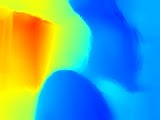
\includegraphics[width=0.8\linewidth]{images/depth_full-depth-image}
        \caption{Full Depth API depth image}
    \end{subfigure}%
    \begin{subfigure}[b]{0.4\textwidth}
        \centering
        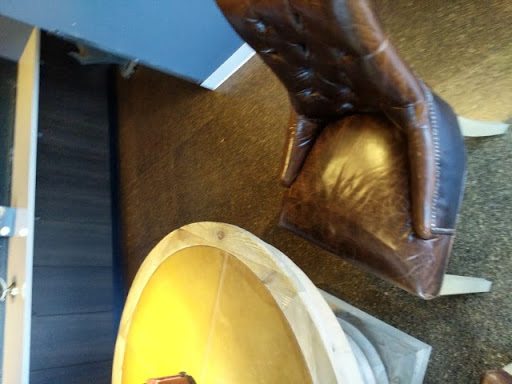
\includegraphics[width=0.8\linewidth]{images/depth_camera-image}
        \caption{Camera image}
    \end{subfigure}%

    % Optional: Adjust or remove vertical spacing between the rows
    \vspace{0.5em}

    % Second row
    \begin{subfigure}[b]{0.4\textwidth}
        \centering
        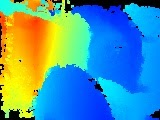
\includegraphics[width=0.8\linewidth]{images/depth_raw-depth-image}
        \caption{Raw Depth API depth image}
    \end{subfigure}%
    \begin{subfigure}[b]{0.4\textwidth}
        \centering
        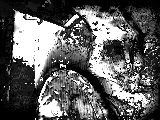
\includegraphics[width=0.8\linewidth]{images/depth_raw-depth-confidence-image}
        \caption{Raw Depth API confidence image}
    \end{subfigure}%

    \caption{Full Depth vs. Raw Depth}
    \label{fig:depth-api-images}
\end{figure}


The Depth API is preferred in cases where it is crucial to have a depth value for every pixel, such as calculating if an object should be occluded by the scene in an AR application,
while the Raw depth API is preferred if accuracy of the depth information is crucial. \parencite{google_llc_arcore_doc}
As accuracy is crucial for primitive detection and depth information for every pixel is not required, the Raw Depth API is used in this project.


\section{Building the point cloud (PC)}
As RANSAC is a point-based algorithm, we first need to convert the depth image to a point cloud.
The process consists of three steps.
\begin{enumerate}
    \item Filtering low confidence points
    \item Transforming depth image pixels to world coordinate points
    \item Inserting new points into the point cloud
\end{enumerate}

\subsection{Filtering low confidence points}
The confidence image provided by the Raw Depth API can be used to filter out points with low confidence.
A threshold value is set, below which points are discarded.

\subsection{Transforming depth image pixels to world coordinate points}
To convert the point into world coordinates, first the camera intrinsics are used to
project the point into camera space.
Then, the model matrix is used to transform the point into world space.
\parencite{google_llc_codelab_raw_depth,google_llc_arcore_doc}

These transformations can be seen as analog to the transformations needed to
render an object in world space onto the screen, as described in section~\ref{sec:rendering-the-primitives}.
In this case, the transformation is applied backwards, i.e.\ in the opposite direction of the arrows
in the figure~\ref{fig:coordinate-systems}, starting from screen space (5) to world space (2).
The parameters for the perspective projection matrix (section~\ref{sec:perspective-projection}) are derived from the camera intrinsics.


%"Given point $A$ on the observed real-world geometry and a 2D point a representing the same point in the depth image,
%the value given by the Depth API at a is equal to the length of $CA$ projected onto the principal axis.
%This can also be referred as the z-coordinate of $A$ relative to the camera origin $C$." \parencite{google_llc_arcore_doc}
%\begin{figure}[h]
%    \centering
%    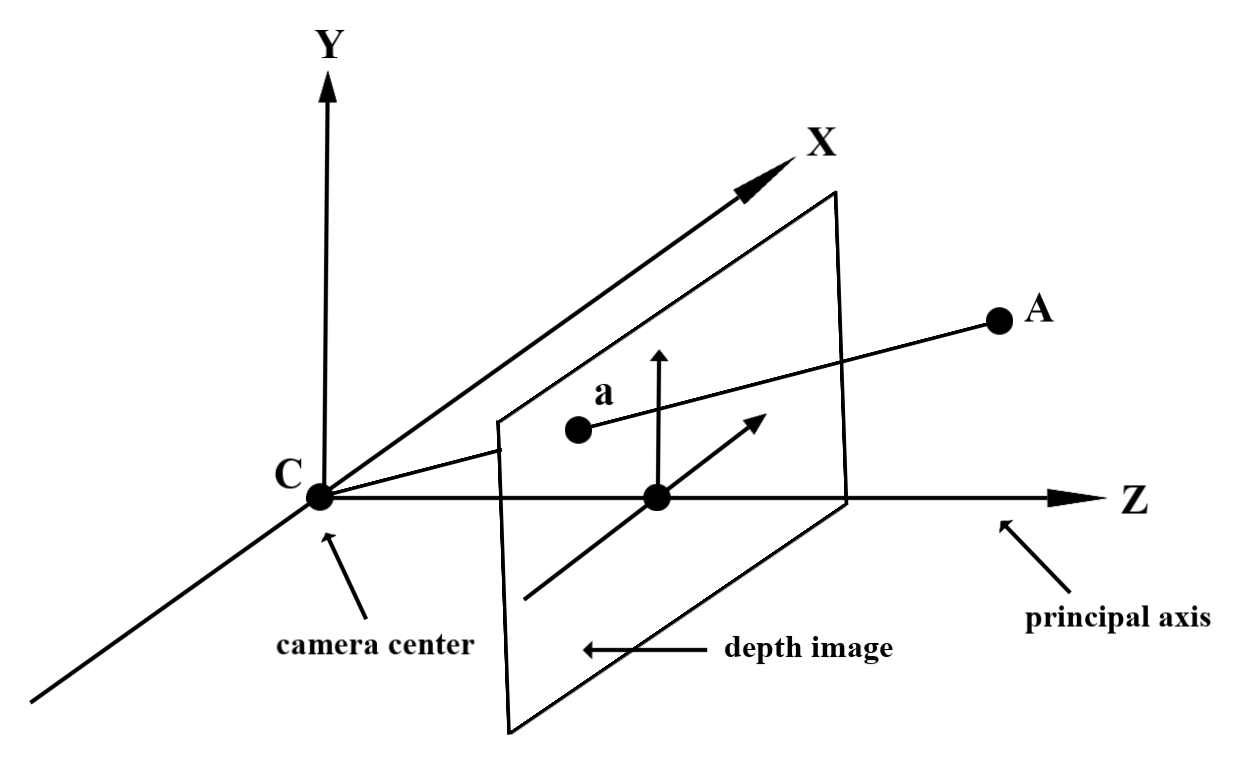
\includegraphics[width=0.75\textwidth]{images/depth-values-diagram}
%    \caption{}
%    \label{fig:}
%\end{figure}
%%codeblock with the formula
%\begin{lstlisting}[language=Java]
%float fx =
%  cameraTextureIntrinsics.getFocalLength()[0] * depthWidth / intrinsicsDimensions[0];
%float fy =
%  cameraTextureIntrinsics.getFocalLength()[1] * depthHeight / intrinsicsDimensions[1];
%float cx =
%  cameraTextureIntrinsics.getPrincipalPoint()[0] * depthWidth / intrinsicsDimensions[0];
%float cy =
%  cameraTextureIntrinsics.getPrincipalPoint()[1] * depthHeight / intrinsicsDimensions[1];
%pointCamera[0] = depthMeters * (x - cx) / fx;
%pointCamera[1] = depthMeters * (cy - y) / fy;
%pointCamera[2] = -depthMeters;
%pointCamera[3] = 1;
%\end{lstlisting}

%This results in a point in camera space,
%which can then be transformed into world space by multiplying it with the model matrix.

\subsection{Inserting new points into the point cloud}

The last step is to add new points to the point cloud.
As new depth images are captured every frame, we can not simply store a list of all points to append the new data to.
This would lead to a massive amount of points that represent the same point in space, with slightly different depth values.
To circumvent this, we can use a data structure that allows us to partition the space into smaller regions, and only store one point per region.
A simple approach would utilize a grid, where each cell represents a region in space, while a more sophisticated approach
would use a spatial data structure like an octree to improve performance.

\paragraph{Octree}
An octree is a tree data structure where each node has exactly eight children.
The tree can be used to sparsely partition three-dimensional space into smaller cubes and allows for efficient
insertion and traversal in logarithmic time.
"For the definition a simple recursive splitting of [cubes] is continued until there is only one point in a [cube]."
\parencite{gabriel_zachmann_geometric_2002}

\begin{figure}[h]
    \centering
    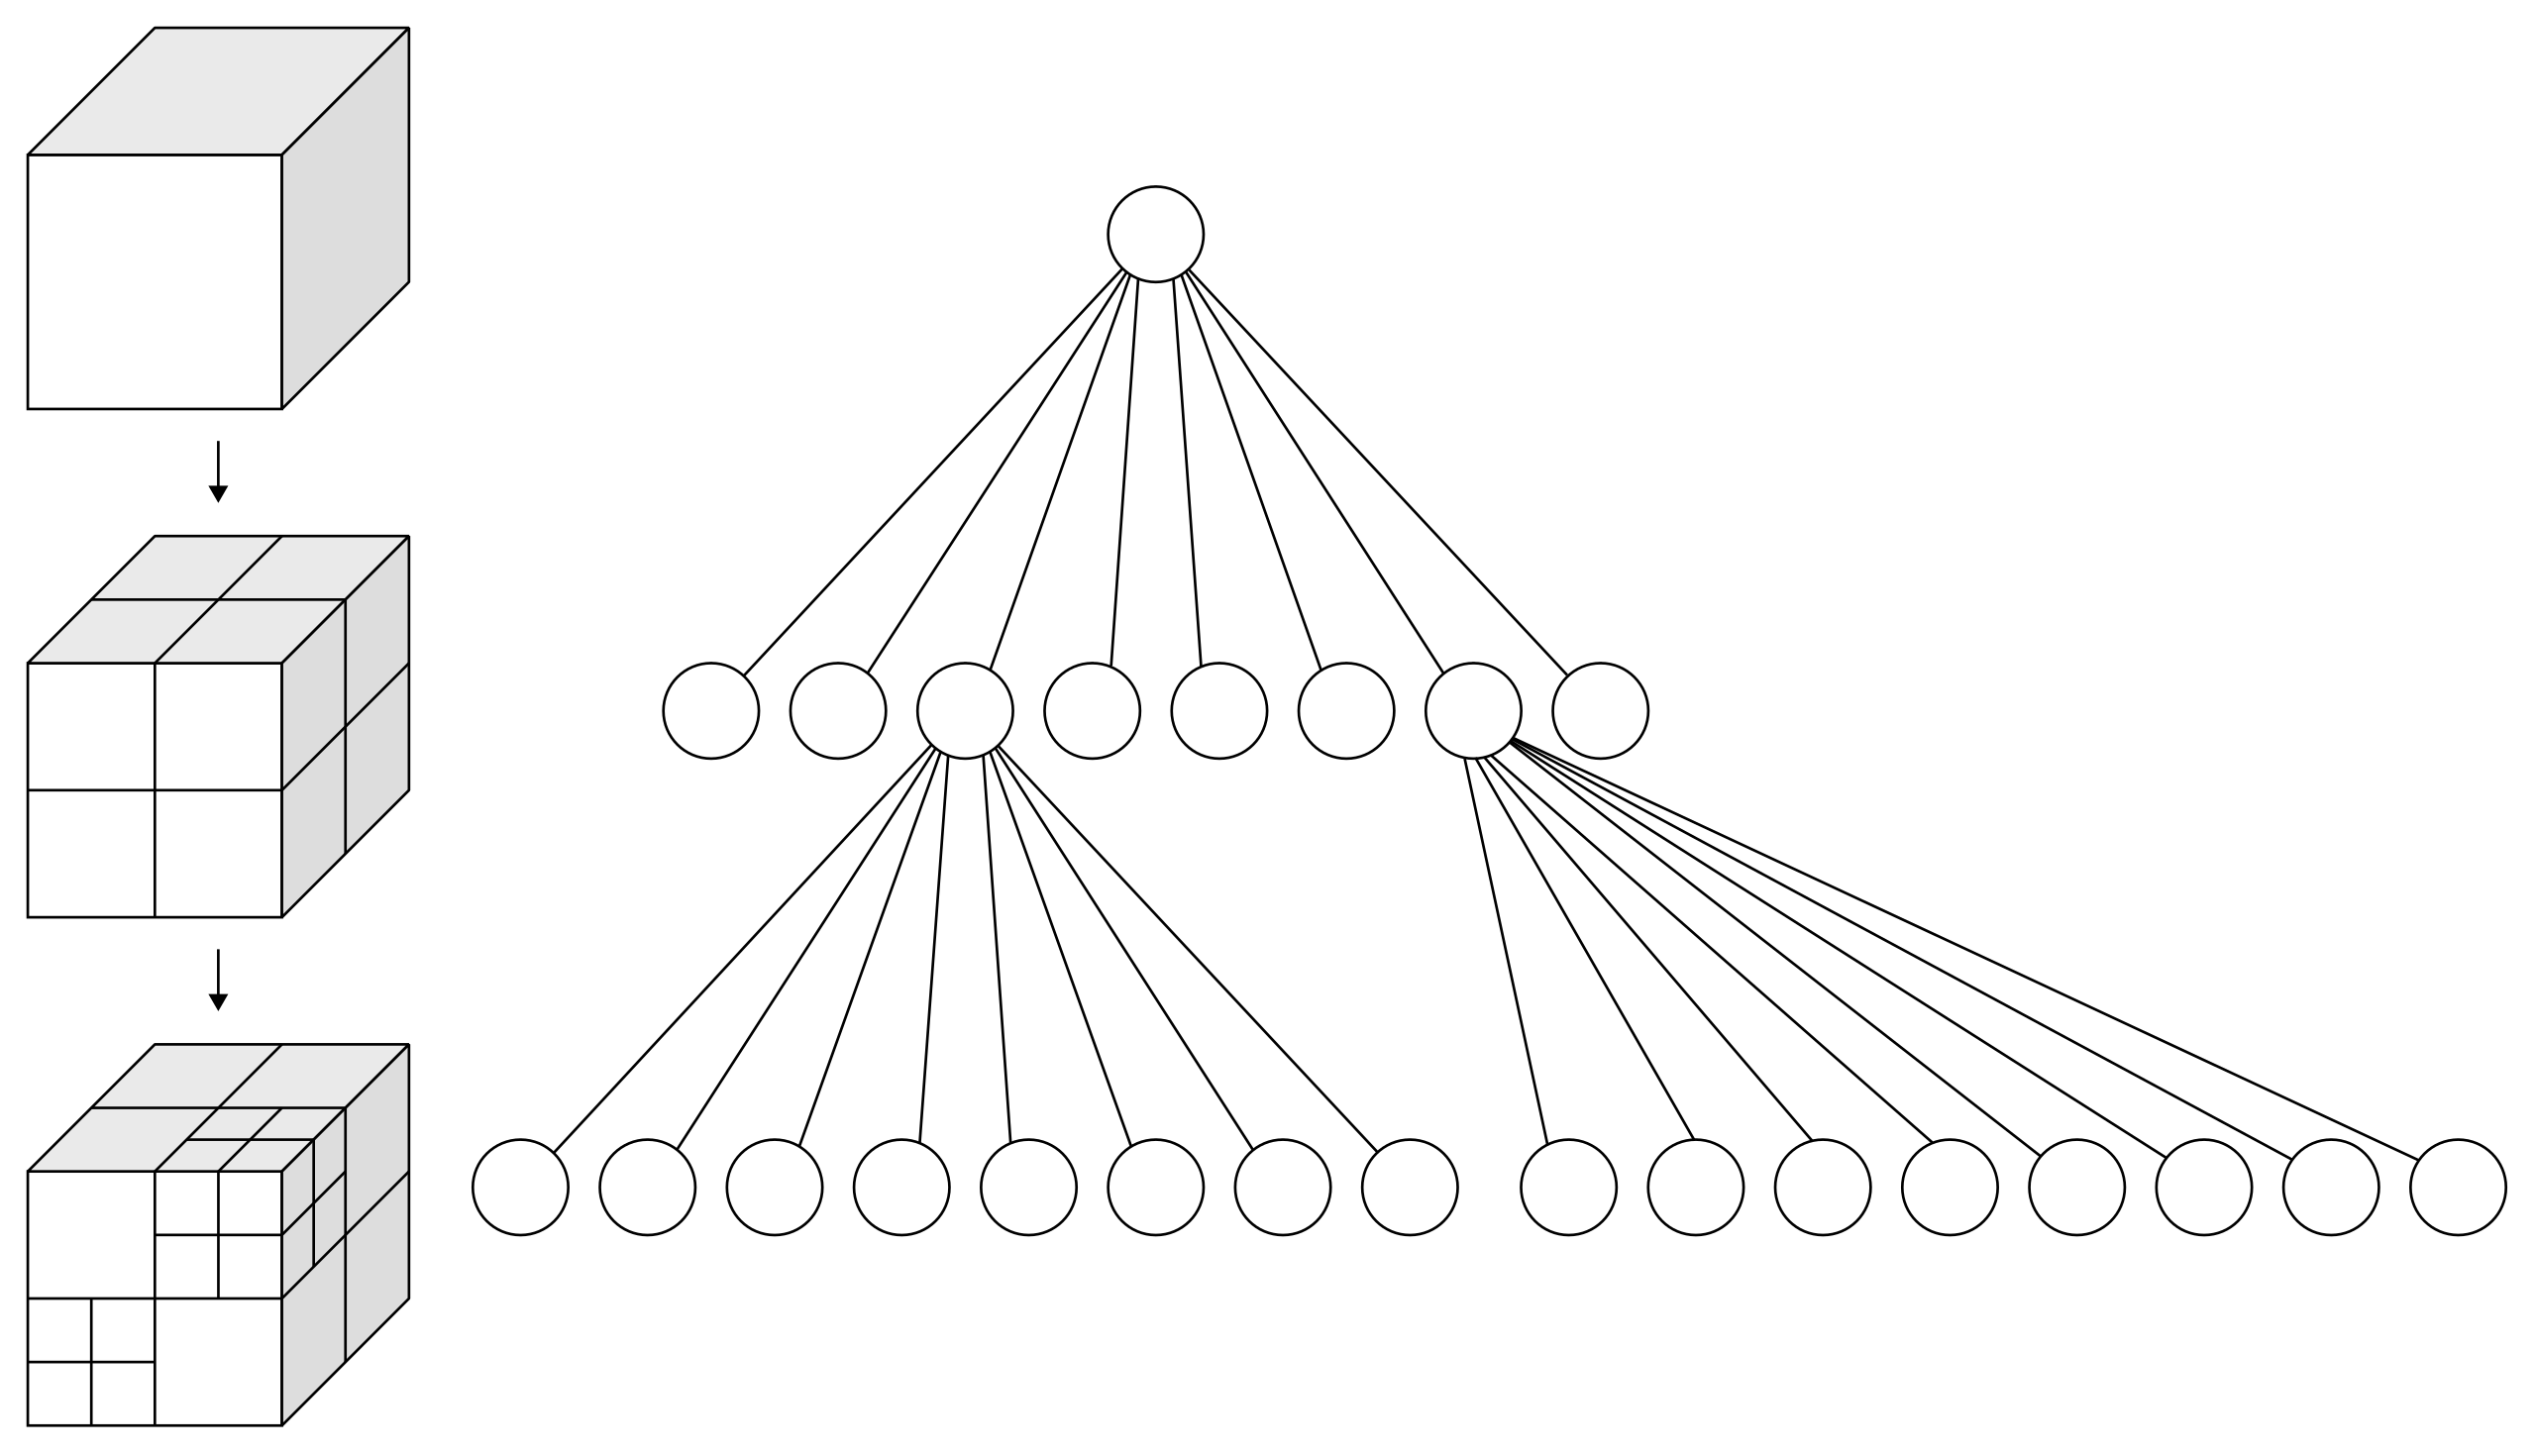
\includegraphics[width=0.75\textwidth]{images/octree}
    \caption{Octree}
    \label{fig:octrree}
\end{figure}

\subsubsection{Fixed Depth Octree}
A straightforward approach to utilize an octree for point cloud storage is to use a variation of the octree with a fixed depth.
Points are always inserted at the defined depth of the tree, creating all nodes up to that depth if they do not yet exist.
The center coordinate of the leaf node can then be inferred as the point in space,
thus saving the coordinates of the point explicitly is not required.
Instead, to find the coordinates of a given node, the tree needs to be traversed while keeping track of
the extent and center coordinate of the current node.
This approach will naturally provide quantization of the point cloud, with the resolution of the point cloud
determined by the depth of the octree and extend of the root .
Using this approach, duplicate points are removed and adjusting the resolution of the octree
allows for fine-tuning of the threshold distance between points under which points are considered duplicates.

One advantage of an octree with a fixed with is simplicity.
The biggest drawback is that the resolution of the point cloud is fixed and needs to be chosen beforehand.
As the accuracy of the depth images differ between devices and other conditions like lighting and texture,
it is difficult to choose a fixed resolution that works for all cases.

When using a resolution that is too high, some surfaces might be detected as multiple surfaces instead of one.
This is due to the same point being detected multiple times with slightly different depth values.
If the uncertainty of the depth data is too high for the chosen resolution,
points representing the same point in space will be added to neighboring cells of the octree.
In the case of planes, this will lead to points in multiple cells across the normal of the plane,
(increasing the thickness of the plane).
The RANSAC algorithm will then detect multiple planes instead of one.

Quantization might also lead to worse detection results for surface that do not align with the axis of the octree.
For example, a plane that is tilted by a couple of degrees will lead to aliasing,
meaning that the distance between the points and the fitted plane will vary across the plane.

\subsubsection{Octree with neighborhood condition}
%todo
To utilize an octree for point cloud storage, the point coordinates and its data is saved in the leaf nodes of the octree.
In this case, each node of the octree saves the coordinate of the point and its confidence value.
When inserting a new point with a certain confidence value, a range query with a radius calculated from the confidence value
is performed to find all nodes within a certain distance of the point to be inserted.
If no node is found, a new leaf node is created and the point is inserted.
If a node is found with a lower confidence value, the new point is inserted and the old node is removed.
If a node is found with a higher confidence value, the new point is not inserted and discarded.
Using this approach, duplicate points are removed and adjusting the multiplier for the radius of the range query
allows for fine-tuning of the threshold under which points are considered duplicates.

To check if an octree node, which is an axis-aligned bounding box (AABB) with equal sides, and a sphere intersect,
the square distance between the center the sphere and the closest point on the AABB is calculated.
If the square distance is smaller than the square of the radius of the sphere, the sphere and the AABB intersect.

Calculating the square distance between a sphere and the closest point on the AABB can be achieved by summing up the
squared distance in each dimension:
If the sphere's center is outside the extent of the box on a given axis,
the distance is the amount by which it exceeds the box's boundary; otherwise, the distance is zero.
In $n$ dimensions, this can be expressed as
\begin{equation}
    d^2 = \sum_{i=1}^{n} \left\{
    \begin{array}{ll}
        (C_i - B_i - s) ^2 & \text{if } C_i > (B_i + s) \\
        (C_i - B_i + s)^2  & \text{if } C_i < (B_i - s) \\
        0                  & \text{otherwise}
    \end{array}
    \right
\end{equation}
where $C$ is the center of the sphere, $B$ is the center of the AABB, and $s$ is the half-size of the AABB\@.
\parencite{glassner_graphicsgems_2013}


\section{Detecting Primitives using RANSAC}

\parencite{schnabel_efficient_2007}


\section{Rendering the primitives}\label{sec:rendering-the-primitives}
The primitives are stored in world space, as in relative to the worlds' origin.
To render the primitives and overlay them onto the camera feed,
transforming the points from world space to screen space is required.

\subsection{OpenGL Rendering Pipeline}
This section provides an overview of the OpenGL rendering pipeline and the necessary steps to render the primitives.
All subsections are based on the book~\citetitle{de_vries_learn_2020} by \citeauthor{de_vries_learn_2020}~\parencite{de_vries_learn_2020}.

\subsubsection{Coordinate Systems}\label{subsec:coordinate-systems}
In OpenGL rendering, five coordinate systems are commonly used, as illustrated in figure~\ref{fig:coordinate-systems}.
In these coordinate systems, coordinates are relative to:
\begin{enumerate}
    \item the objects origin (\textit{Local Space})
    \item the worlds origin (\textit{World Space})
    \item the cameras origin (\textit{View Space})
    \item the cameras origin (\textit{Clip Space}) with visible coordinates between -1 and 1 in all dimensions (frustum).
    Coordinates outside the frustum are clipped.
    Perspective projection can be applied here, more details in the next subsection.
    \item the screen (\textit{Screen Space})  with the origin in the bottom left corner of the screen
\end{enumerate}
To transform vertices between these systems, their positions are multiplied with a corresponding transformation matrix.
One exception is the viewport transformation,
which is applied by OpenGL automatically based on the viewport settings provided via the \texttt{glViewport} function.

\begin{figure}[h!]
    \centering
    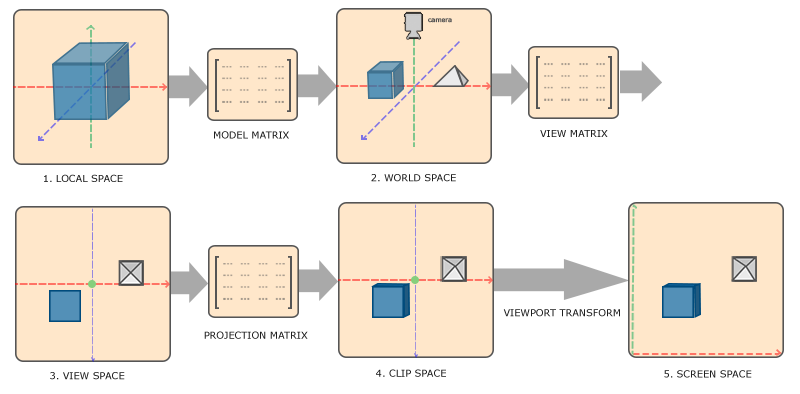
\includegraphics[width=\linewidth]{images/coordinate_systems}
    \caption{Coordinate systems}
    \label{fig:coordinate-systems}
\end{figure}

\subsubsection{Perspective Projection}\label{sec:perspective-projection}
In the real world, objects appear smaller the further away they are from the viewer.
To simulate this effect in 3D rendering, perspective projection is used.
Perspective projection is achieved through the use of homogeneous coordinates,
which are an extension of the Cartesian coordinate system.
In homogeneous coordinates, each point in 3D space is represented by four coordinates instead of three: $(x, y, z, w)$.

The transformation from 3D space to a 2D projection is handled by a projection matrix.
This matrix is designed to map the viewable scene, defined within a specified frustum, to a normalized cube known as clip space.
The frustum is a truncated pyramid shape that represents the volume of space visible through the camera lens.
The parameters of the frustum are defined by the field of view, aspect ratio, and near and far clipping planes,
as illustrated by figure~\ref{fig:perspective}
\begin{figure}[h]
    \centering
    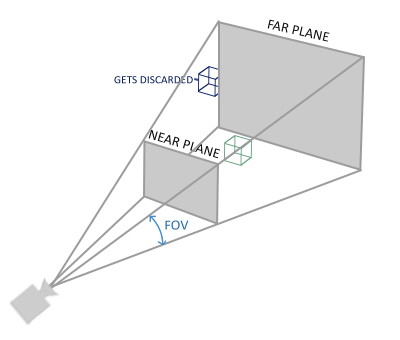
\includegraphics[width=0.50\textwidth]{images/perspective}
    \caption{Perspective Projection}
    \label{fig:perspective}
\end{figure}

"The projection matrix [\ldots] also manipulates the w value of each vertex coordinate in such a way
that the further away a vertex coordinate is from the viewer, the higher this w component becomes"~\parencite{de_vries_learn_2020}.
When the coordinates are later divided by $w$ (a process known as the perspective divide), %TODO QUOTAION NEEDED
it results in the desired perspective scaling effect.
Points closer to the viewer have a smaller $w$ and are less affected by the divide,
while points further away have a larger $w$ and are reduced in size more significantly

\subsubsection{Shaders}\label{subsec:shaders}
Shaders are isolated programs that run on the GPU and can be used to render objects.
In OpenGL, they are written in the OpenGL Shading Language (GLSL).

Two types of shaders are required to render an object: Vertex shaders and fragment shaders.

Vertex shaders are executed for each vertex defined in the vertex buffer, which is defined on the CPU and
passed to the GPU by copying the data to the GPU's memory, e.g.\ by using the \texttt{glBufferData} function.
A vertex shader can be used to transform the vertices from model space to screen space using the
model, view, and projection matrices.
To achieve this, the Model-View-Projection matrix (MVP) matrix can be passed as a \textit{uniform} to the vertex shader,
which means it is the same for all vertices.
The MVP matrix is the result of multiplying the model matrix, view matrix, and projection matrix.
As the MVP matrix is the same for all vertices of an object, it can be calculated on the CPU and passed to the GPU as a uniform.
The vertex position is then multiplied by the MVP matrix to transform it into clip space.
The resulting position is then passed to the fragment shader by assigning it to the \texttt{gl\_Position} variable.

\begin{figure}[h]
    \centering
    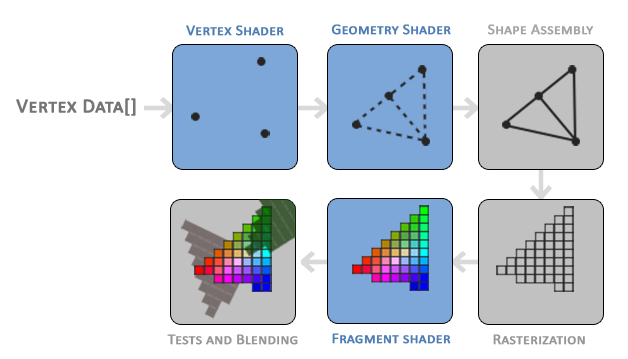
\includegraphics[width=0.70\textwidth]{images/graphics-pipeline}
    \caption{Graphics Pipeline. Blue boxes represent programmable stages. The Geometry Shader is optional and not covered in this thesis.}
    \label{fig:graphics-pipeline}
\end{figure}


The graphics pipeline then rasterizes and interpolates the vertex positions alongside all other vertex attributes
across the primitive, which are then passed to the fragment shader, which is executed for each pixel the primitive covers.
The fragment shader then outputs the color of the pixel by setting the \texttt{out vec4 FragColor} variable.
Before the final color is written to the framebuffer,
a depth test is performed to determine if the pixel is visible or covered by other pixels from other primitives.

\subsection{Rendering planes}
The RANSAC algorithm provides the parameterization of any detected plane using a normal vector $n$ and the point $p$ relative the worlds origin.
Using OpenGL, a plane can be rendered by creating two triangles composed of 3 vertices each, with two corner vertices shared between the triangles.
To render a plane from the parameterization, one can first find any two vectors $u$ and $v$
that are perpendicular to each-other and to the normal vector $n$.
Using $u$ and $v$, the four vertices of the plane can then be calculated by adding and subtracting $u * size / 2$ and $v * size / 2$ from the point $p$.

\paragraph{Calculating an arbitrary perpendicular vector}
The cross product of two vectors $a$ and $b$ is a vector that is perpendicular to both $a$ and $b$,
as long as $a$ and $b$ are not parallel.
To calculate an arbitrary perpendicular vector to a given vector $n$, one can use any of the 3 basis vectors ${b_1}$, ${b_2}$, and ${b_3}$.
Choosing any of the basis vectors that is not parallel to $n$ will result in a perpendicular vector.
To minimize floating point errors, which are largest for planes where $n$ almost aligns with the chosen basis vector,
the basis vector with the smallest dot product with $n$ can be chosen.
The normalized cross product of two vectors $n$ and $b_{smallest}$ then yields a perpendicular vector to $n$.

\begin{figure}[ht!]
    \centering
    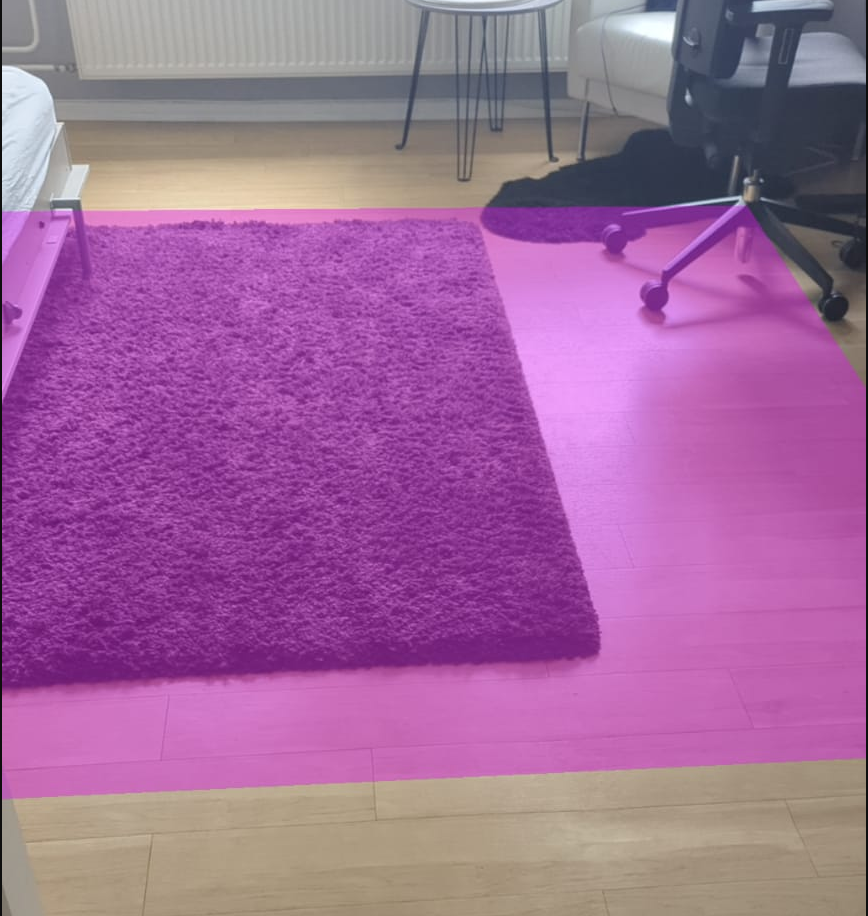
\includegraphics[width=0.6\linewidth]{images/renderedPlane}
    \caption{Rendered RANSAC plane with size of 2*2m}
\end{figure}

\subsection{Constraining the primitives to the area where the points are located}
To constrain the primitive to the area where the points are located, multiple approaches can be used.
One would be to calculate the maximum and minimum values of the points in each dimension and use these to create a bounding box for the plane.
A more sophisticated approach would be to calculate the convex hull of the points to constrain the plane.

The convex hull of a set of points is the smallest convex polygon that contains all the points. %TODO: Citation needed

To render a plane constrained by the convex hull,
a triangle mesh can be created with triangles consisting of two subsequent triangles of the hull vertices and the centroid of the hull as the third vertex each.
Figure~\ref{fig:convex-hull} shows the result of the convex hull algorithm applied to a real dataset of a plane.

\begin{figure}[ht!]

    \centering
    \begin{subfigure}[b]{0.4\textwidth}
        \centering
        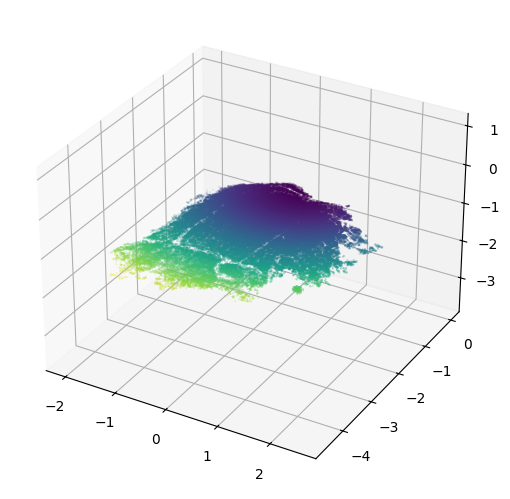
\includegraphics[width=\linewidth]{python/plots/hull/points}
        \caption{Point data}
    \end{subfigure}%
    \begin{subfigure}[b]{0.4\textwidth}
        \centering
        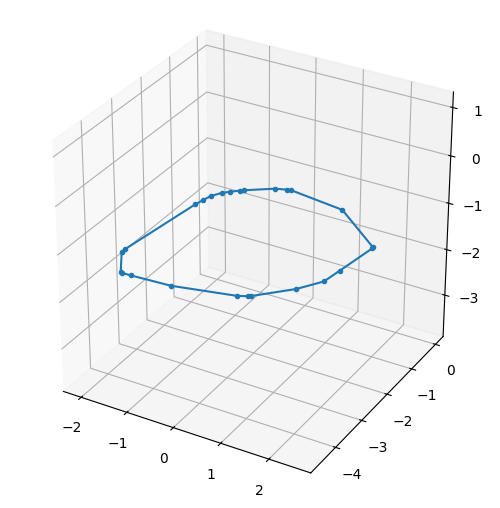
\includegraphics[width=\linewidth]{python/plots/hull/hull}
        \caption{Convex Hull}
    \end{subfigure}%

    \vspace{0.5em}

    \begin{subfigure}[b]{0.8\textwidth}
        \centering
        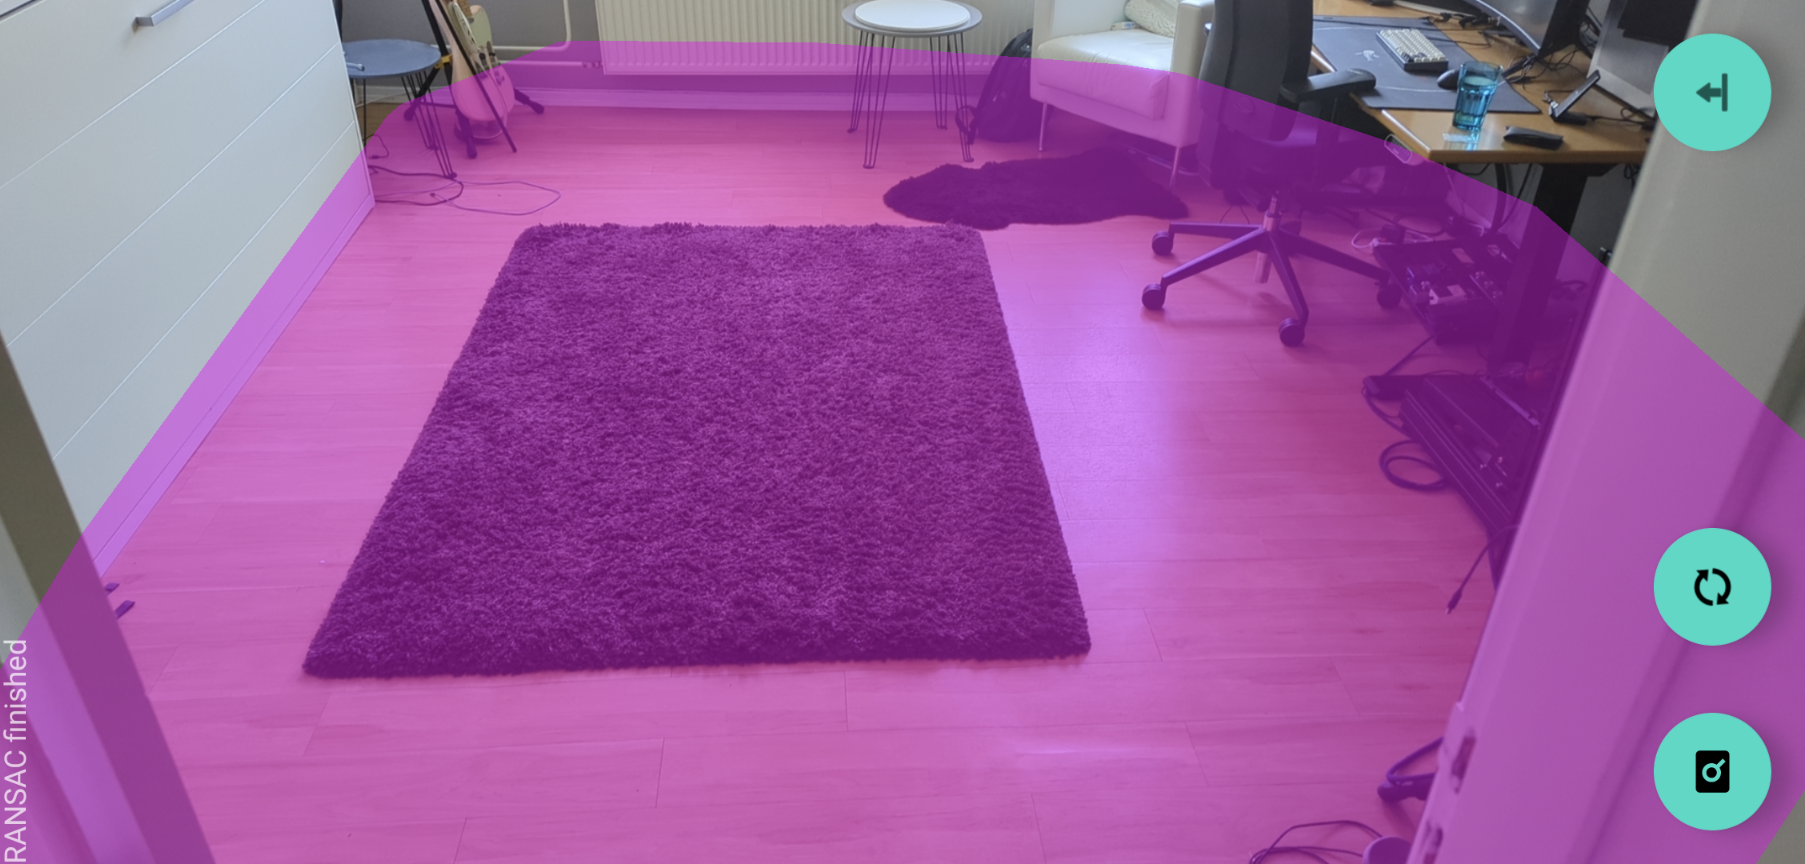
\includegraphics[width=\linewidth]{images/hull}
        \caption{Rendered Primitive}
    \end{subfigure}%
    \caption{Convex Hull with real data}
    \label{fig:convex-hull}
\end{figure}





\parencite{graham_efficient_1972}
\parencite{andrew_another_1979}

\subsection{Preparing the data on the CPU}

\subsubsection{Restraining the primitives}

\paragraph{Cross-section => Floor and Walls}

\paragraph{Using a bounding box / extend of points}

\subsubsection{Building a mesh}

\subsection{Rendering on the GPU (shaders)}

\chapter{Evaluation}\label{ch:evaluation}
In this chapter, the individual algorithms, as well as the final performance of the combined system, will be evaluated.
The depth from motion algorithm will be evaluated based on different materials and their resulting confidence maps in section~\ref{sec:eval-depth-from-motion}.
In section~\ref{sec:eval-ransac-algorithm}, the RANSAC algorithm will be evaluated based on synthetic data, as well as real world data.
Finally, in section~\ref{subsec:application-performance-of-full-room-scan}, the application performance will be evaluated on the use case of a full room scan.
CloudCompare~\cite{daniel_girardeau-montaut_cloudcompare_nodate}, an open-source tool for working with 3D point clouds, will be used for the evaluation of the point clouds and the RANSAC algorithm.
%klare begründung => Anforderung erfüllt ja oder nein

\section{Depth from Motion}\label{sec:eval-depth-from-motion}
As the depth from motion algorithm greatly differs in its performance based on the amount of texture in the captured scene~\cite{google_llc_arcore_doc},
this section will evaluate different materials based on their resulting confidence maps, as retrieved from the ARCore Raw Depth API\@.
In figure~\ref{fig:materials}, the confidence maps of different materials are shown - the camera image on top, the confidence map on the bottom.

\begin{figure}[h!tb]
    \centering
    % First row
    \begin{subfigure}[b]{0.25\textwidth}
        \centering
        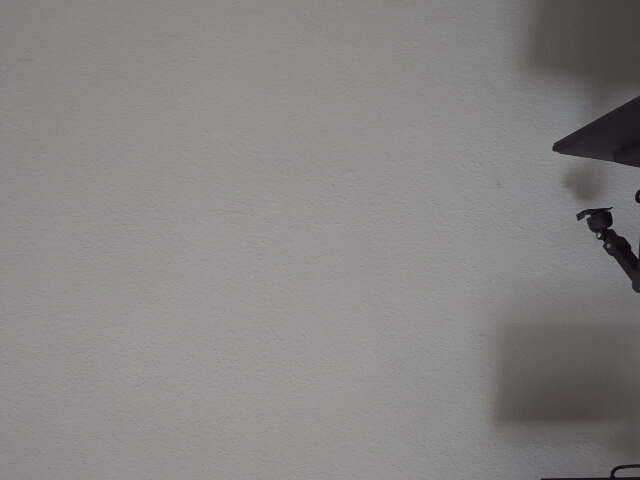
\includegraphics[width=0.9\linewidth]{images/materials/wall-far-cam}
    \end{subfigure}%
    \begin{subfigure}[b]{0.25\textwidth}
        \centering
        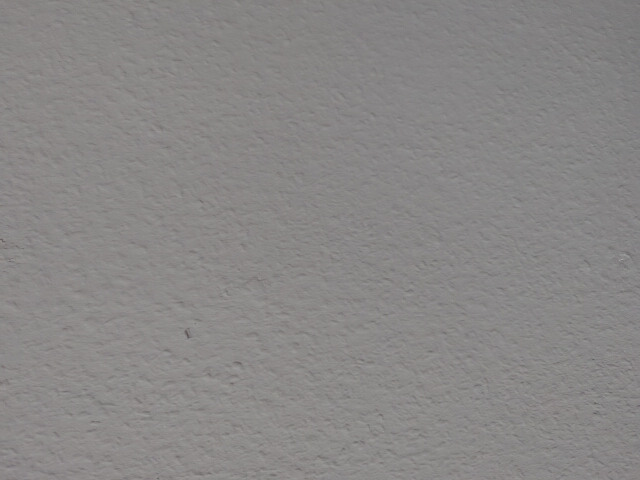
\includegraphics[width=0.9\linewidth]{images/materials/wall-close-cam}
    \end{subfigure}%
    \begin{subfigure}[b]{0.25\textwidth}
        \centering
        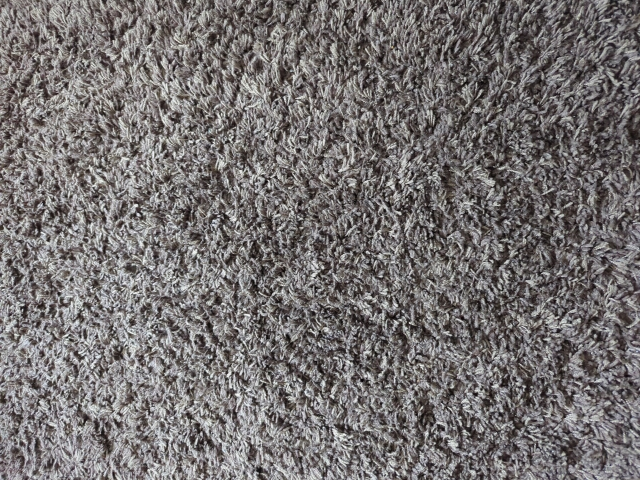
\includegraphics[width=0.9\linewidth]{images/materials/carpet-cam}
    \end{subfigure}%
    \begin{subfigure}[b]{0.25\textwidth}
        \centering
        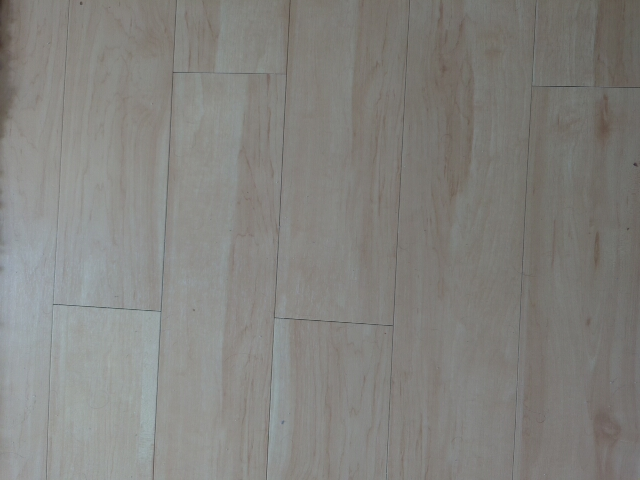
\includegraphics[width=0.9\linewidth]{images/materials/wood-cam}
    \end{subfigure}%

    \begin{subfigure}[b]{0.25\textwidth}
        \centering
        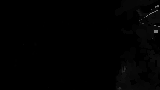
\includegraphics[width=0.9\linewidth]{images/materials/wall-far-conf}
        \caption{Wall, 1.5m}
        \label{fig:material-wall-far}
    \end{subfigure}%
    \begin{subfigure}[b]{0.25\textwidth}
        \centering
        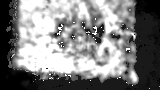
\includegraphics[width=0.9\linewidth]{images/materials/wall-close-conf}
        \caption{Wall, 0.5m}
        \label{fig:material-wall-close}
    \end{subfigure}%
    \begin{subfigure}[b]{0.25\textwidth}
        \centering
        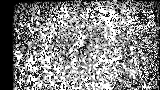
\includegraphics[width=0.9\linewidth]{images/materials/carpet-conf}
        \caption{Carpet}
        \label{fig:material-carpet}
    \end{subfigure}%
    \begin{subfigure}[b]{0.25\textwidth}
        \centering
        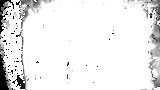
\includegraphics[width=0.9\linewidth]{images/materials/wood-conf}
        \caption{Wooden floor}
        \label{fig:material-wood}
    \end{subfigure}%

    \vspace{0.5em}

    % First row
    \begin{subfigure}[b]{0.25\textwidth}
        \centering
        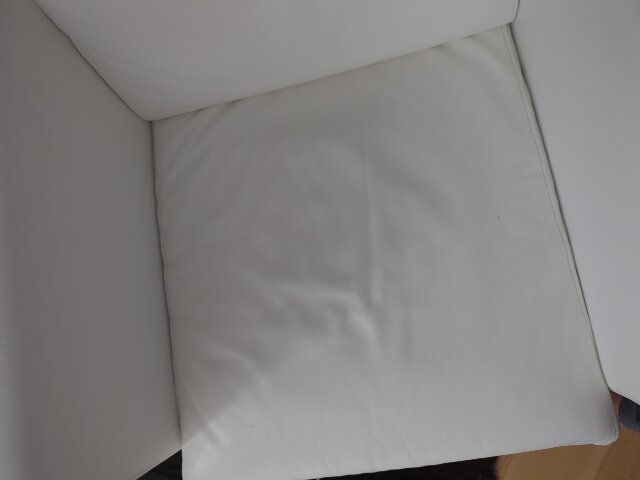
\includegraphics[width=0.9\linewidth]{images/materials/leather-cam}
    \end{subfigure}%
    \begin{subfigure}[b]{0.25\textwidth}
        \centering
        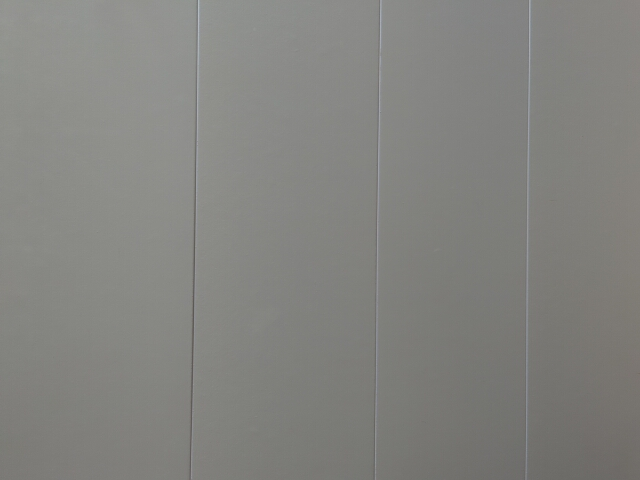
\includegraphics[width=0.9\linewidth]{images/materials/whiteFurniture-cam}
    \end{subfigure}%
    \begin{subfigure}[b]{0.25\textwidth}
        \centering
        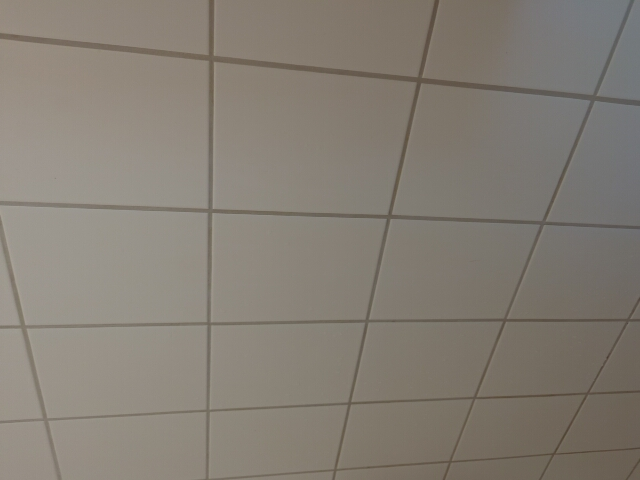
\includegraphics[width=0.9\linewidth]{images/materials/tiles-cam}
    \end{subfigure}%
    \begin{subfigure}[b]{0.25\textwidth}
        \centering
        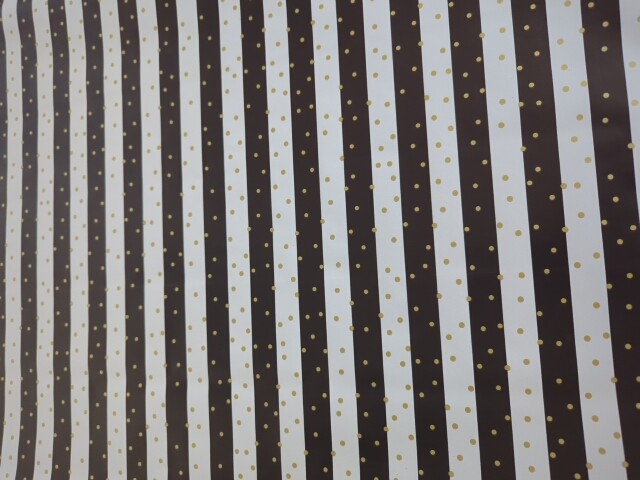
\includegraphics[width=0.9\linewidth]{images/materials/giftpaper-cam}
    \end{subfigure}%

    \begin{subfigure}[b]{0.25\textwidth}
        \centering
        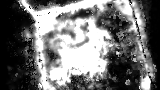
\includegraphics[width=0.9\linewidth]{images/materials/leather-conf}
        \caption{Leather armchair}
        \label{fig:material-leather}
    \end{subfigure}%
    \begin{subfigure}[b]{0.25\textwidth}
        \centering
        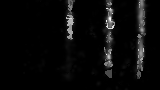
\includegraphics[width=0.9\linewidth]{images/materials/whiteFurniture-conf}
        \caption{White furniture}
        \label{fig:material-whiteFurniture}
    \end{subfigure}%
    \begin{subfigure}[b]{0.25\textwidth}
        \centering
        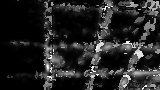
\includegraphics[width=0.9\linewidth]{images/materials/tiles-conf}
        \caption{Bathroom tiles}
        \label{fig:material-tiles}
    \end{subfigure}%
    \begin{subfigure}[b]{0.25\textwidth}
        \centering
        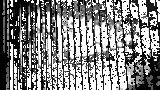
\includegraphics[width=0.9\linewidth]{images/materials/giftpaper-conf}
        \caption{Gift paper}
        \label{fig:material-giftpaper}
    \end{subfigure}%

    \caption{Comparison of confidence maps of different materials. Camera image on top, confidence map on bottom.}
    \label{fig:materials}
\end{figure}

In figure~\ref{fig:material-wall-close} and~\ref{fig:material-wall-far}, the confidence maps of a wall at different distances is shown.
It is apparent that the confidence of the wall at 1.5m distance is almost completely black, meaning low confidence.
This is due to the lack of any texture on the wall at this distance.
When moving closer to the wall, the structure of the wall becomes more apparent and the confidence increases greatly.

In figure~\ref{fig:material-carpet}, a carpet with a lot of texture is shown, the resulting confidence map has fairly high confidence on average,
but also has dark sports throughout the map.
This could be a result of the repetitive pattern of the carpet.

The highest confidence of all tested materials is achieved on a wooden floor, as shown in figure~\ref{fig:material-wood}.
This can be attributed to the high amount of texture and value variance through the wood, while not being repetitive.
The seams between the wooden planks are also clearly visible.

Figure~\ref{fig:material-leather} shows a leather armchair, which has a high confidence on the seams of the chair and
on creases of the leather, with low confidence in other areas, where the leather is smoother.
A similar pattern is visible on white furniture and bathroom tiles, in figures~\ref{fig:material-whiteFurniture} and~\ref{fig:material-tiles} respectively,
where the white surface has very low confidence, while the seams between the surfaces have increased confidence.
The gift paper shown in figure~\ref{fig:material-giftpaper} shows a similar effect, but less pronounced.
As the surface itself is striped with dots randomly placed throughout, the confidence is higher overall,
but the striped pattern is still visible in the confidence map, as the stripes themselves contain little texture.

These examples show how the amount of texture on a given surface greatly influences the confidence of the depth from motion algorithm, as expected.
The algorithm performs best on surfaces with high texture, while struggling with low texture surfaces.
Small repetitive patterns can also lead to low confidence, as visible in the carpet example.
It is also important to note that the texture captured by the camera itself is important, not the texture of the material itself.
This can be seen in the first example of the wall: When capturing from afar, the cameras resolution is too low to capture the texture,
but when moving closer to the wall, the texture of the wall becomes more apparent and the confidence increases.
Lighting conditions will also influence the confidence of the algorithm,
as angled light will create shadows that will increase the texture of the surface~\cite{google_llc_arcore_doc} (not shown in the comparison).

\section{Point Clouds}\label{sec:point-clouds}
This section will evaluate the two point cloud datastructures as described in section~\ref{subsec:inserting-new-points-into-the-point-cloud}.
To evaluate the datastructures, the point cloud is transferred from the mobile application to a computer using
a simple HTTP server with a single endpoint, that accepts a file using a POST request and saves it to disk.
The android application will then stream the point cloud data, serialized as a PLY file, to the server on a push of a button.
A PLY file is a simple file format for storing 3D point cloud data in plain text
and allows for saving custom properties for each vertex, such as the confidence value of the point.
In all the following images of the point clouds, the confidence value is color-coded,
with green being high confidence and red being low confidence.

\begin{lstlisting}[caption=Example PLY file]
ply
format ascii 1.0
element vertex 6
property float x
property float y
property float z
property float confidence
property uchar red
property uchar green
property uchar blue
end_header
0.1851168 -0.77074146 -0.92582846 1.0 0 255 0
-0.061887983 -0.7755803 -0.79551744 1.0 0 255 0
-0.058628604 -0.7638883 -0.7860476 0.80784315 245 10 0
-0.07720285 -0.75610626 -0.80394375 0.81960785 230 25 0
-0.19774273 -0.6645372 -2.5003948 1.0 0 255 0
-0.09499544 -0.028413996 -2.553247 0.99607843 5 250 0
\end{lstlisting}

%\begin{lstlisting}[caption=HTTP server code, language=Python]
%from fastapi import FastAPI
%from starlette.requests import Request
%
%app = FastAPI()
%
%@app.post("/upload")
%async def upload(request: Request):
%    body = await request.body()
%    body_str = body.decode('utf-8')
%    with open("data.ply", "w") as f:
%        f.write(body_str)
%\end{lstlisting}

\begin{figure}[h!tbp]
    \centering
    \begin{subfigure}[b]{0.33\textwidth}
        \centering
        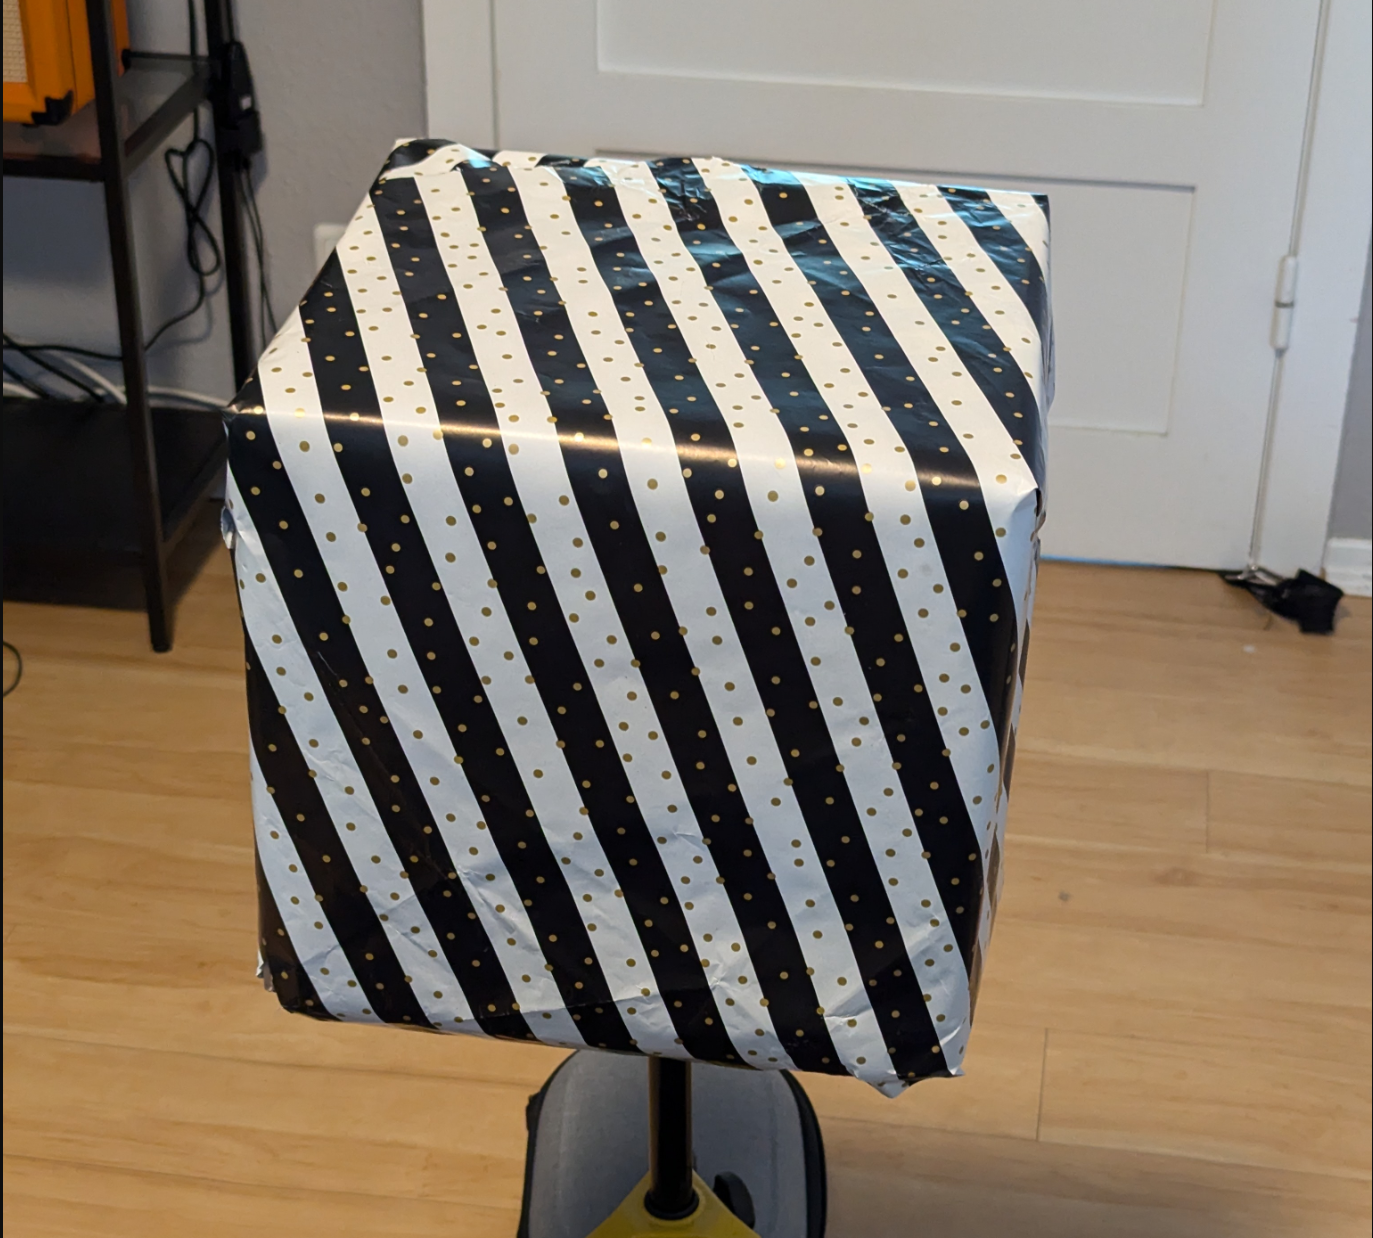
\includegraphics[width=0.9\linewidth]{images/test-setup}
        \caption{Color image of setup}
    \end{subfigure}%
    \begin{subfigure}[b]{0.33\textwidth}
        \centering
        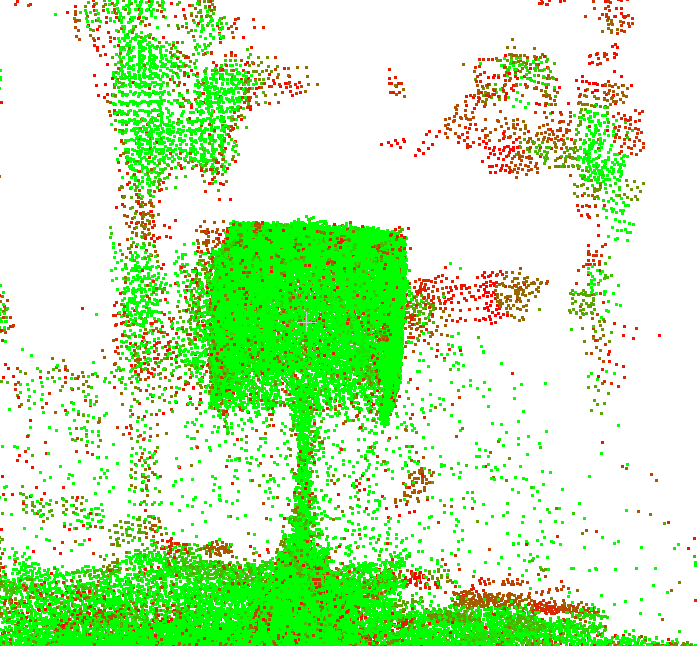
\includegraphics[width=0.9\linewidth]{images/test-setup-cloud}
        \caption{Captured point cloud}
    \end{subfigure}%
    \begin{subfigure}[b]{0.33\textwidth}
        \centering
        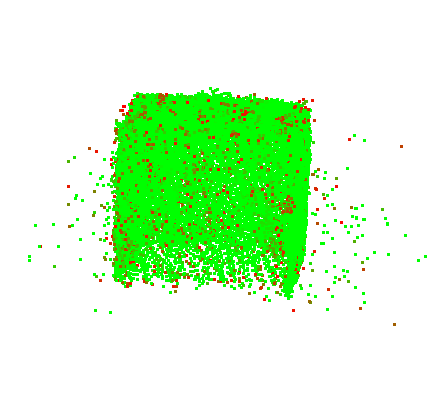
\includegraphics[width=0.9\linewidth]{images/test-setup-segmented}
        \caption{Segmented point cloud}
    \end{subfigure}%
    \caption{Test setup for capturing point clouds}
    \label{fig:test-setup}
\end{figure}

For test data, a cube wrapped with the same gift-paper as in figure~\ref{fig:material-giftpaper} is used, called \textit{test cube} from now on.
The bottom of the test cube is hollow, so in total, 5 faces are visible.
The cube is propped up on stand, to allow for easy segmentation of the point cloud later on,
in order to remove the floor and other objects from the point cloud.
Reproducibility is ensured by using controlled lighting conditions and a fixed setup.
To capture a scan of the test cube, the camera is moved around the cube 3 times, while also moving the camera up and down,
to capture multiple angles for the depth from motion algorithm to work to its full potential.
The full setup is shown in figure~\ref{fig:test-setup}.

\subsection{Quantization Octree vs. Epsilon Octree}\label{subsec:quantization-octree-vs.-epsilon-octree}

A point cloud with a resolution of $s=0.005$m or 5mm is captured for both the quantization octree and the epsilon octree.
The resulting segmented point cloud, the quantization octree has a total of about 90.000 points,
while the epsilon octree only has about 20.000 points.
This can be explained due to the quantization octree always ending up with the maximal resolution
with enough data added, as it is functionally a grid.
The epsilon octree, on the other hand, will only add points that are within the epsilon threshold of the current point,
which means that gaps between points are at least epsilon wide, but can be wider.
For example, if two points almost 2 epsilon apart, no points will be added between them and the gap will be approximately
2 epsilon wide.
As epsilon is set to $s$, the epsilon octree will have fewer points than the quantization octree with the same resolution.
To compare the two datastructures, the quantization octree will be used with a lower resolution of $s=0.010$m,
which results in a number of points of about 22.000, which is comparable to the epsilon octree at $s=0.005$m.

Figure~\ref{fig:octrees-compairison} shows the raw and segmented point clouds of both datastructures.
From inspecting the raw point cloud visually, it is apparent that the quantization octree has a higher amount of noise,
While the cube is easily recognizable in the epsilon octree point cloud, the quantization octree point cloud has a lot of noise around the cube.
The quantization octree also has more low-confidence points than the epsilon octree.
This is due to the quantization octree always adding points to the cloud that fall within the threshold,
while the epsilon octree only adds / updates points based on a condition that takes the confidence of the point into account
and ignores points lower confidence points that are close to higher confidence points.
As such, the epsilon octree improves the accuracy of the point cloud when new, higher confidence points are added.


\begin{figure}[h!tb]
    \centering
    \begin{subfigure}[b]{0.4\textwidth}
        \centering
        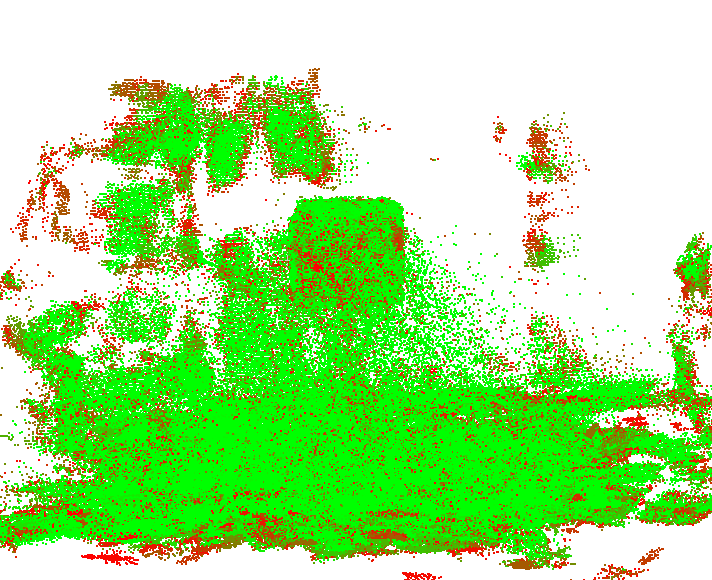
\includegraphics[width=0.9\linewidth]{images/eval-clouds-quant2}
    \end{subfigure}%
    \begin{subfigure}[b]{0.4\textwidth}
        \centering
        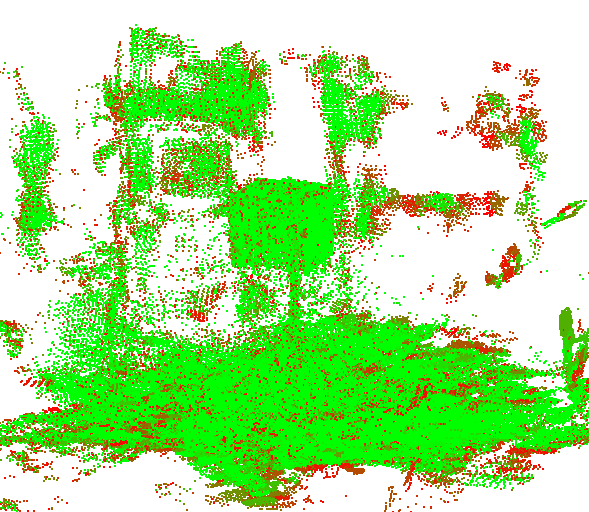
\includegraphics[width=0.9\linewidth]{images/eval-clouds-epsilon}
    \end{subfigure}%

    \begin{subfigure}[b]{0.4\textwidth}
        \centering
        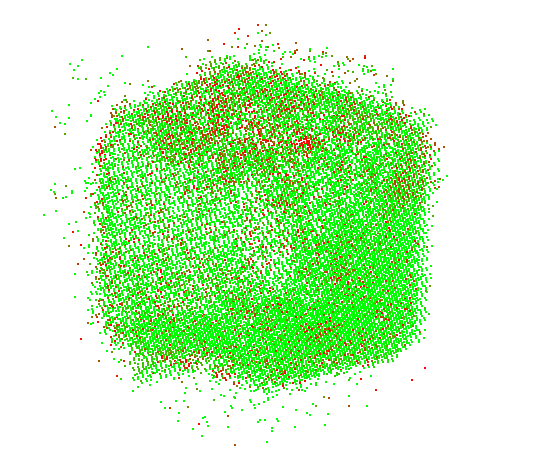
\includegraphics[width=0.9\linewidth]{images/eval-clouds-quant-segmented2}
        \caption{Quantization Octree, $s=0.010$m}
    \end{subfigure}%
    \begin{subfigure}[b]{0.4\textwidth}
        \centering
        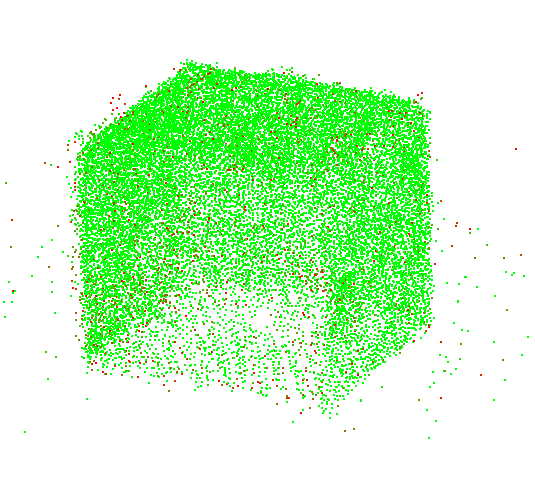
\includegraphics[width=0.9\linewidth]{images/eval-clouds-epsilon-segmented}
        \caption{Epsilon Octree, $s=0.005$m}
        \label{fig:octrees-compairison-epsilon}
    \end{subfigure}%

    \caption{Comparison of Quantization Octree and Epsilon Octree. Raw point cloud on top, segmented on bottom.}
    \label{fig:octrees-compairison}
\end{figure}

To calculate statistics on the point clouds, the real box is measured and a primitive box with matching dimensions is created in CloudCompare.
Using the \textit{fine registration (ICP)} feature, it is possible to align the point clouds to the primitive box.
The underlying algorithm of the fine registration feature is the Iterative Closest Point (ICP) algorithm,
which iteratively minimizes the mean square distance between a "model" shape and a "data" shape~\cite{besl_method_1992}.
Once the point clouds are aligned to the primitive,
the distance between the points of the point cloud and the primitive box can be calculated using the \textit{Cloud/Mesh Distance} feature in CloudCompare.
The result of this calculation can be seen in figure~\ref{fig:octrees-compairison-stats}.
From the histogram, it is apparent that the quantization octree has higher noise than the epsilon octree.
This can also bee seen in the standard deviation, which is 0.022 for the quantization octree and 0.011
for the epsilon octree.
This confirms the first suspicion from visual inspection of the point clouds.
The mean distance is also higher for the quantization octree, with 0.0046 compared to 0.0011 for the epsilon octree.
This can be understood as points being 0.5cm and 0.1cm away from the real surface in mean, respectively.
If these points were to be used for primitive detection, this would indicate how far off the detected primitives would be from the real surface.

These results suggest that the epsilon octree is an improvement over the quantization octree in terms of accuracy,
both when it comes to the amount of noise and the distance to the real surface.

\begin{figure}[h!tbp]
    \centering
    \begin{subfigure}[b]{0.5\textwidth}
        \centering
        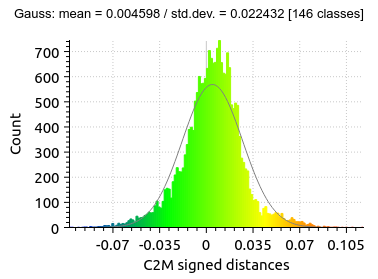
\includegraphics[width=0.9\linewidth]{images/eval-quant-hist}
        \caption{Quantization Octree}
    \end{subfigure}%
    \begin{subfigure}[b]{0.5\textwidth}
        \centering
        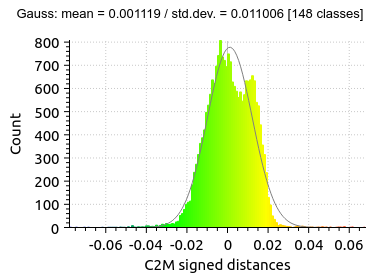
\includegraphics[width=0.9\linewidth]{images/eval-epsilon-hist}
        \caption{Epsilon Octree}
    \end{subfigure}%
    \caption{Histogramm of distances between segmented point cloud points and primitive mesh}
    \label{fig:octrees-compairison-stats}
\end{figure}

\section{RANSAC Algorithm}\label{sec:eval-ransac-algorithm}
In this section, the RANSAC algorithm will be evaluated based on a model of a cube,
first using synthetic data in section~\ref{subsec:tests-on-singular-synthetic-cube} and then using real world data
in section~\ref{subsec:ransac-tests-on-real-world-data}.

\subsection{Tests on Synthetic Cube}\label{subsec:tests-on-singular-synthetic-cube}

A unit cube will be used as a test object to evaluate the RANSAC algorithm.
The cube has been generated with a side length of 1 and a sampling rate of 0.01.
This would equate to a cube with a side length of 1m and a distance of 1cm between points in the real world,
which is comparable to what was used in section~\ref{subsec:quantization-octree-vs.-epsilon-octree}.

\subsubsection{Resilience to Noise}
In figure~\ref{fig:test-noise}, the unit cube is shown with varying noise levels using gaussian noise.
The noise level is defined as the standard deviation of the noise added to the points.

With a noise level of 0.01, the cube is perfectly reconstructed.
Increasing the noise level to 0.02, the cube is still recognized mostly correctly.
Starting from noise level to 0.03, the default parameters do not yield correct results.
To achieve correct results, the epsilon parameter of the RANSAC algorithm has to be increased to 0.2.
This leads to 6 faces being recognized correctly, but some points not being assigned to the correct faces,
as the with each primitive extraction pass, points are extracted that lie within 0.2 of the recognized plane.


\begin{figure}[h!tbp]
    \centering
    % First row
    \begin{subfigure}[b]{0.25\textwidth}
        \centering
        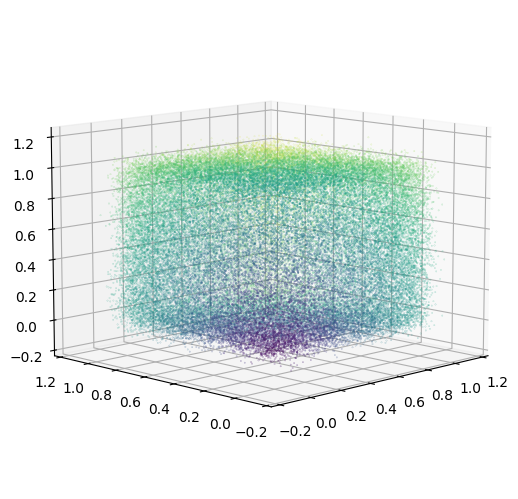
\includegraphics[width=0.9\linewidth]{python/plots/cube_points/data/cube_points}
    \end{subfigure}%
    \begin{subfigure}[b]{0.25\textwidth}
        \centering
        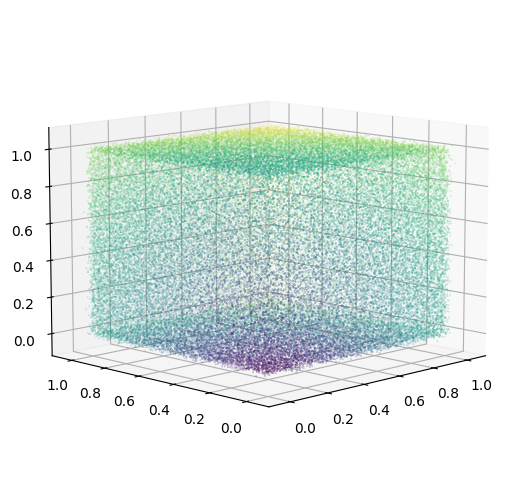
\includegraphics[width=0.9\linewidth]{python/plots/cube_points/data/noise/cube_points_noise_01}
    \end{subfigure}%
    \begin{subfigure}[b]{0.25\textwidth}
        \centering
        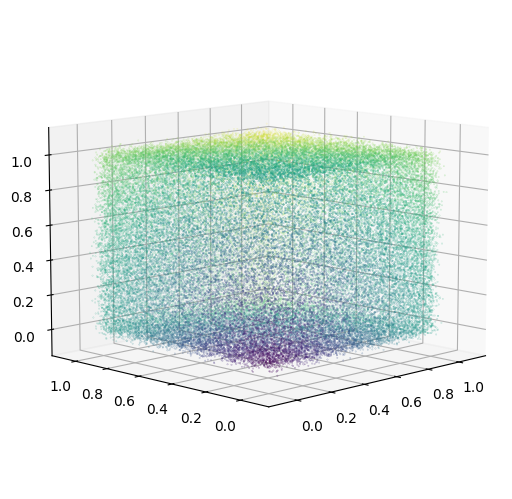
\includegraphics[width=0.9\linewidth]{python/plots/cube_points/data/noise/cube_points_noise_02}
    \end{subfigure}%
    \begin{subfigure}[b]{0.25\textwidth}
        \centering
        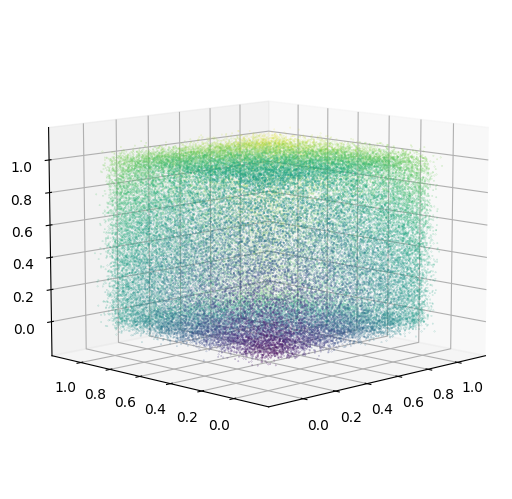
\includegraphics[width=0.9\linewidth]{python/plots/cube_points/data/noise/cube_points_noise_03}
    \end{subfigure}%

%    \vspace{0.5em}

    \begin{subfigure}[b]{0.25\textwidth}
        \centering
        
\includegraphics[width=0.9\linewidth]{python/plots/cube_points/data/cube_points_primitives}
        \caption{Noise level 0.00}
    \end{subfigure}%
    \begin{subfigure}[b]{0.25\textwidth}
        \centering
        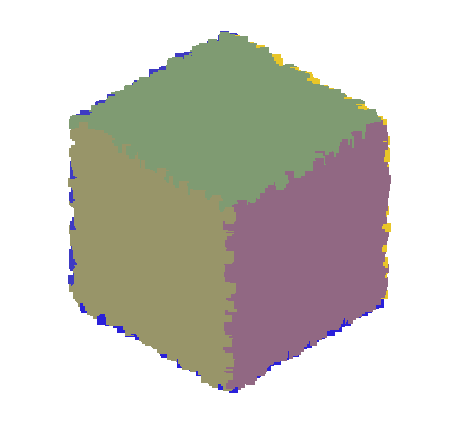
\includegraphics[width=0.9\linewidth]{python/plots/cube_points/data/noise/cube_points_noise_01_primitives}
        \caption{Noise level 0.01}
    \end{subfigure}%
    \begin{subfigure}[b]{0.25\textwidth}
        \centering
        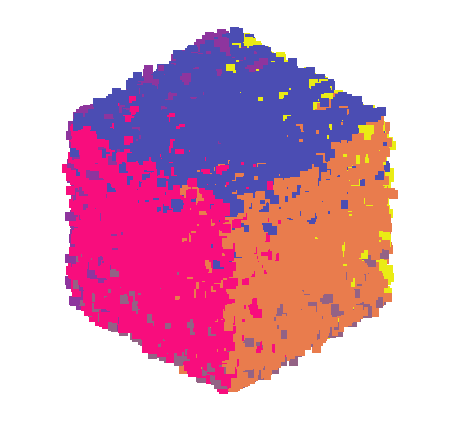
\includegraphics[width=0.9\linewidth]{python/plots/cube_points/data/noise/cube_points_noise_02_primitives}
        \caption{Noise level 0.02}
    \end{subfigure}%
    \begin{subfigure}[b]{0.25\textwidth}
        \centering
        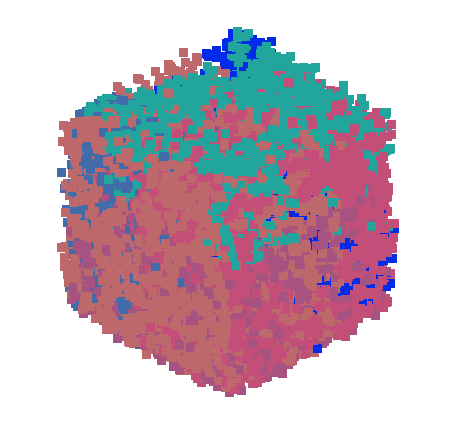
\includegraphics[width=0.9\linewidth]{python/plots/cube_points/data/noise/cube_points_noise_03_primitives}
        \caption{Noise level 0.03}
    \end{subfigure}%

    \caption{Unit cube with varying noise level}
    \label{fig:test-noise}
\end{figure}

\subsubsection{Resilience to Missing Data}

As a big problem of depth from motion techniques is the lack of depth information in areas with minimal texture,
the resilience to missing data is crucial.
In figure~\ref{fig:test-missing}, points towards the center of the cubes surfaces have been removed.
This mimics the structure of real world data from the Depth API,
as edges are often detected more accurately than surfaces.
%TODO: citation needed
To achieve this, points have been removed with an increasing probability based on the
quadratic distance to the center of the face the points belongs to.

The algorithm is able to correctly recognize the faces of the cube with a missing level up to 24.
With a missing level of 48, the algorithm still detects the planes, but doesn't assign all points to the faces.
With increasing missing level, the n parameter, which defines the minimum number of points required to fit a primitive,
is also required to be lowered.
In real world applications this would lead to more false detections, primitives being detected where there are none.

%Given a point $x$ with coordinates $(x_1, x_2, x_3)$, edge length $l$, and missing data rate $r$,
%the distance to the closest edge can be calculated as |
%
%As the cube is centered at the origin and aligned with the axis, the absolute of one coordinate will always equal $l/2$.
%By filtering out this coordinate, the point $x$ can be projected onto the plane of the cube,
%resulting in point $x'$ with coordinates $(x'_1, x'_2)$.
%
%The probability $p$ of a point being removed can then be calculated as

%\begin{equation}
%    p = \left(\frac{\sqrt{(l/2 - |x'_1|) \cdot (l/2 - |x'_2|)}}{l / 2}\right)^2 \cdot r
%\end{equation}

\begin{figure}[h!tbp]
    \centering
    % First row
    \begin{subfigure}[b]{0.25\textwidth}
        \centering
        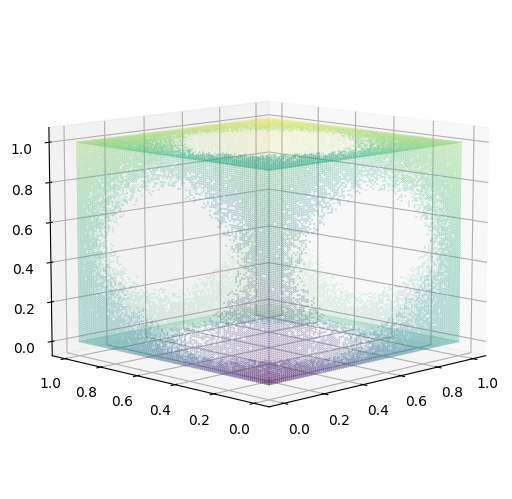
\includegraphics[width=0.9\linewidth]{python/plots/cube_points/data/missing/cube_points_missing_6_0}
    \end{subfigure}%
    \begin{subfigure}[b]{0.25\textwidth}
        \centering
        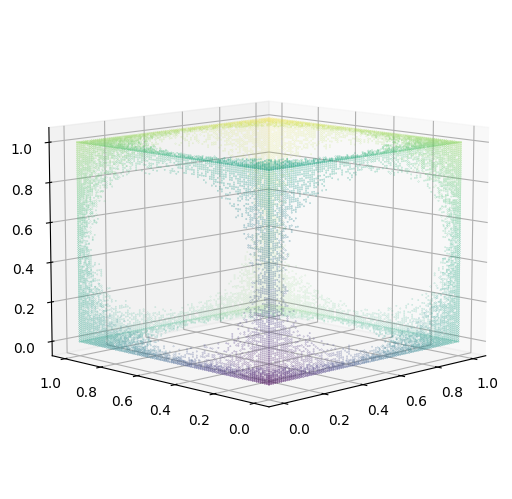
\includegraphics[width=0.9\linewidth]{python/plots/cube_points/data/missing/cube_points_missing_12}
    \end{subfigure}%
    \begin{subfigure}[b]{0.25\textwidth}
        \centering
        \includegraphics[width=0.9\linewidth]{python/plots/cube_points/data/missing/cube_points_missing_24}
    \end{subfigure}%
    \begin{subfigure}[b]{0.25\textwidth}
        \centering
        \includegraphics[width=0.9\linewidth]{python/plots/cube_points/data/missing/cube_points_missing_48}
    \end{subfigure}%

%    \vspace{0.5em}

    \begin{subfigure}[b]{0.25\textwidth}
        \centering
        \includegraphics[width=0.9\linewidth]{python/plots/cube_points/data/missing/cube_points_missing_6_primitives}
        \caption{Missing level 6}
    \end{subfigure}%
    \begin{subfigure}[b]{0.25\textwidth}
        \centering
        \includegraphics[width=0.9\linewidth]{python/plots/cube_points/data/missing/cube_points_missing_12_primitives}
        \caption{Missing level 12}
    \end{subfigure}%
    \begin{subfigure}[b]{0.25\textwidth}
        \centering
        \includegraphics[width=0.9\linewidth]{python/plots/cube_points/data/missing/cube_points_missing_24_primitives}
        \caption{Missing level 24}
    \end{subfigure}%
    \begin{subfigure}[b]{0.25\textwidth}
        \centering
        \includegraphics[width=0.9\linewidth]{python/plots/cube_points/data/missing/cube_points_missing_48_primitives}
        \caption{Missing level 48}
    \end{subfigure}%

    \caption{Unit cube with varying missing level}
    \label{fig:test-missing}
\end{figure}

\subsubsection{Resilience to Noise and Missing Data Combined}

When combining both noise and missing data, the quality of the detection is much worse.
In figure~\ref{fig:test-both}, the cube is shown with a noise level of 0.01 and varying missing levels.
With noise level 0.01 and missing level 6, the cube is still recognized correctly.
With missing level 12, more than 6 faces are being recognized, but all the points are still assigned to primitives.
This is explained by the fact that the parameterization of the planes is not accurate enough to fit all the points of the planes.
Thus, the algorithm only fits a subset of the points to the primitive and will create a new parameterization
for the remaining points.
To achieve results with these conditions, the epsilon parameter had to be increased to 0.015 to achieve any results at all.
Using a noise level of 0.02 with missing data yields no satisfactory results, even with tweaking the parameters.

\begin{figure}[ht!]

    \centering
    % First row
    \begin{subfigure}[b]{0.25\textwidth}
        \centering
        \includegraphics[width=0.9\linewidth]{python/plots/cube_points/data/matrix/cube_points_m6_n01}
    \end{subfigure}%
    \begin{subfigure}[b]{0.25\textwidth}
        \centering
        \includegraphics[width=0.9\linewidth]{python/plots/cube_points/data/matrix/cube_points_m12_n01}
    \end{subfigure}%
    \begin{subfigure}[b]{0.25\textwidth}
        \centering
        \includegraphics[width=0.9\linewidth]{python/plots/cube_points/data/matrix/cube_points_m24_n01}
    \end{subfigure}%

%    \vspace{0.5em}

    \begin{subfigure}[b]{0.25\textwidth}
        \centering
        \includegraphics[width=0.9\linewidth]{python/plots/cube_points/data/matrix/cube_points_m6_n01_primitives}
        \caption{Missing level 6}
    \end{subfigure}%
    \begin{subfigure}[b]{0.25\textwidth}
        \centering
        \includegraphics[width=0.9\linewidth]{python/plots/cube_points/data/matrix/cube_points_m12_n01_primitives}
        \caption{Missing level 12}
    \end{subfigure}%
    \begin{subfigure}[b]{0.25\textwidth}
        \centering
        \includegraphics[width=0.9\linewidth]{python/plots/cube_points/data/matrix/cube_points_m24_n01_primitives}
        \caption{Missing level 24}
    \end{subfigure}%
    \caption{Unit cube with noise level = 0.01 and varying missing level}
    \label{fig:test-both}

\end{figure}

\subsection{Tests on Real World Data}\label{subsec:ransac-tests-on-real-world-data}

Figure~\ref{fig:real-data-ransac} show the results of the RANSAC algorithm on the dataset created with the epsilon octree,
as seen in figure~\ref{fig:octrees-compairison-epsilon}.
Note that CloudCompare uses AABBs to represent the planes, instead of the convex hull as used in the application.
In the segmented dataset, the cube is recognized correctly, with all 5 faces being recognized.
In the raw dataset, the faces of the cubes are still recognized, but the algorithm also recognizes other planes in the dataset,
some of which contain a subset of the points of the cube.
This shows a limitation of the RANSAC algorithm, which is similar to~\cite{tarsha-kurdi_hough-transform_2007} findings,
where plane primitives are constructed from points which do not belong to the same plane.
\cite{schnabel_efficient_2007} solution to this problem is using a bitmap to detect connected shapes, as mentioned in section~\ref{subsec:schnabels-efficient-ransac-algorithm}.
Only the largest connected shape in a given shape candidate is kept.
As the points that are not part of the largest connected shape are kept in the dataset, the algorithm will still consider them in the next iterations.
However, if the resulting separate primitives then do not cross the support threshold, they are filtered out.
In other words, the bitmap epsilon parameter $\beta$ can be used to adjust the resolution of the bitmap,
with higher values leading to shapes being detected as separate shapes quicker, while the minimum support threshold $n$
can be used to filter out shapes that are not supported by enough points.

\begin{figure}[htb]
    \centering

    \begin{subfigure}[b]{0.5\textwidth}
        \centering
        \includegraphics[width=0.7\linewidth]{images/results_cube}
        \caption{Segmented dataset, default parameters}
        \label{fig:real-data-ransac-segmented}
    \end{subfigure}%

    \vspace{0.5em}

    \begin{subfigure}[b]{0.5\textwidth}
        \centering
        \includegraphics[width=0.7\linewidth]{images/results_all}
        \caption{Raw dataset, $n=400, \epsilon=0.024, \beta=0.047$}
    \end{subfigure}%
    \begin{subfigure}[b]{0.5\textwidth}
        \centering
        \includegraphics[width=0.7\linewidth]{images/results-all-2}
        \caption{Raw dataset, $n=400, \epsilon=0.024, \beta=0.005$}
    \end{subfigure}%
    \caption{RANSAC results on real data set collected using the epsilon octree}
    \label{fig:real-data-ransac}
\end{figure}

In the case of the dataset visible in figure~\ref{fig:real-data-ransac},
the default value of the bitmap epsilon parameter was set to $\beta=0.024$.
Ideally, the bitmap epsilon parameter would be set to the sample resolution of the dataset~\parencite{schnabel_efficient_2007}.
When raising the resolution to $\beta=0.005$, the detection results of the cube are improved,
while still detecting some artifacts that shouldn't be detected.
With these parameters, the planes in the background are also no longer detected,
as their effective sampling resolution is too low, which causes them to be detected as many separate shapes that do not cross the support threshold.
This shows that applying the algorithm to a dataset with vastly varying sampling resolutions will
lead to suboptimal results, as the parameters need to be set for the whole dataset.
This is problematic for the use case in combination with the depth from motion algorithm, as the Raw Depth API
will have low confidence in areas with low texture, which will cause lower sampling rates, or completely missing data,
which will in turn lead to connected shapes not being present and being filtered out.
It is therefore difficult to find a parameterization for the algorithm that fits both highly textured and low-textured objects.


\subsection{Application Performance}\label{subsec:application-performance-of-full-room-scan}

This section will evaluate the combined performance of the application, first on the test cube, then on a full room scan.

\subsubsection{Test Cube}
Figure~\ref{fig:cube-results} shows the results of a scan of the test cube, under the same procedure as in section~\ref{sec:point-clouds}.
Note that the point cloud is not segmented in the application, thus other planes (namely the floor) are also detected in the background.

With an epsilon octree resolution of $s=0.015$, one of the faces is merged with points from the stand the cube is placed on.
Starting with a resolution of $s=0.010$, all the 5 faces are recognized correctly and
the convex hull algorithm correctly creates a matching polygon for each face, however there are still small gaps between the faces.
Increasing the resolution further to $s=0.005$ improves the accuracy of the edges of the planes slightly.
While there are no longer gaps between the faces, some amount of clipping is now visible in the polygons.
%With the selected parameters, a total of 250.000 points were collected and processed by the RANSAC algorithm in about 20 seconds.

\begin{figure}[h!tbp]
    \centering

    \begin{subfigure}[b]{\textwidth}
        \centering
        \includegraphics[width=0.3\linewidth]{images/cube_015_1}
        \includegraphics[width=0.3\linewidth]{images/cube_015_2}
        \includegraphics[width=0.3\linewidth]{images/cube_015_3}
        \caption{$s=0.015, n\approx60.000$}
    \end{subfigure}%

    \vspace{0.5em}

    \begin{subfigure}[b]{\textwidth}
        \centering
        \includegraphics[width=0.3\linewidth]{images/cube_010_1}
        \includegraphics[width=0.3\linewidth]{images/cube_010_2}
        \includegraphics[width=0.3\linewidth]{images/cube_010_3}
        \caption{$s=0.010, n\approx125.000$}
    \end{subfigure}%

    \vspace{0.5em}

    \begin{subfigure}[b]{\textwidth}
        \centering
        \includegraphics[width=0.3\linewidth]{images/cube_005_1}
        \includegraphics[width=0.3\linewidth]{images/cube_005_2}
        \includegraphics[width=0.3\linewidth]{images/cube_005_3}
        \caption{$s=0.005, n\approx250.000$}
    \end{subfigure}%

    \caption{Detection results of the test cube using the mobile application}
    \label{fig:cube-results}
\end{figure}

Using a trial-and-error approach, the parameters of the RANSAC algorithm were adjusted to achieve the best trade-off between
performance, the amount of detected planes and noise.
The final parameters used are:
\begin{itemize}
    \item $0.010>s>0.005$ -- The resolution of the epsilon octree.
    Higher resolutions than 0.005 lead to a significantly higher amount of points and thus worse runtime performance without noticeable improvements in the detection results,
    while lower resolutions than 0.010 lead to visibly worse results, with outliers having a bigger impact on the detection results, as visible in figure~\ref{fig:cube-results}.
    \item $n=\left(\frac{1}{s}\right)^2\cdot0.15^2=900$ -- The minimum number of points required to fit a primitive.
    Equal to the amount of points on a $15cm^2$ plane, if uniformly sampled with $s$.
    Realistically, this number will be lower, as the points are scattered across the normal of the plane.
    However, the epsilon octree also has a lower actual resolution than $s$, as discussed in section~\ref{subsec:quantization-octree-vs.-epsilon-octree},
    which should cancel out the effect.
    The calculation is only a rough estimate and proved to show good results.
    \item $\epsilon=0.022$ -- The epsilon parameter of the RANSAC algorithm.
    Lower values lead to planes being detected as multiple planes along the planes normal.
    This parameter varies depending on noise of the data.
    Two standard deviations contain 95.5 percent of all data, which is used as a starting point.
    As the epsilon octree showed a standard deviation of 0.011, a value of 0.022 is chosen and shows good results.
    \item $\beta=1.5s$ -- The epsilon parameter of the bitmap.
    As discussed in~\ref{subsec:ransac-tests-on-real-world-data}, settings this parameter is a trade of between detecting shapes that have missing data and filtering out shapes that are not connected in reality.
    $1.5s$ is a rather strict value that filters out most shapes with gaps in their data due to missing texture, however it greatly reduces the amount of artifacts.
\end{itemize}
Other parameters are kept at their default values.
As all parameters except $\epsilon$ are relative to $s$,
it should be easy to adapt the parameters to different devices that might offer depth maps with other accuracies -
only the resolution of the epsilon octree has to be adjusted.
As for $\epsilon$, the parameter needs to be adjusted based on the noise level of the data, which might vary based on the device and the lighting conditions.


As for runtime performance, the device remains responsive with $\epsilon<0.005$, however the device heats
up quickly and the application experiences a significant slowdown after a few scans.
This is due to both the creation of the point cloud using the epsilon octree and the RANSAC algorithm being
very computationally expensive.

\subsubsection{Full Room Scan}

Figure~\ref{} shows the results of a full room scan.


\chapter{Conclusion and Outlook}

\section{Future Work}

The system developed in this thesis provides a foundation for further research and development in
the field of processing depth data from ARCore or similar APIs that provide a sequence of depth images, to create a mesh of a scene.
However, the biggest current limitation of the system is the quality of the depth data, as the depth-from-motion technique
used by ARCore has limitations when it comes to detecting depth in objects with minimal texture.

An interesting aspect for further research is thus exploring the data quality of different devices,
with and without depth sensors, and how it affects the performance of the primitive detection algorithm.
Using the Full Depth API instead of the Raw Depth API and testing if the interpolated depth data improves the results
is also a valid point of further research.

As far as extending the system, implementing the detection of more complex primitives,
such as cylinders and spheres, would be a logical next step.
The part of detecting the actual primitives also provides a good starting point for further research,
as there exist many different algorithms, specialized for different types of contexts and applications, as discussed in chapter~\ref{ch:primitive-detection-algorithms}.
As the system provides the foundation for building the point cloud and rendering the primitives,
it is possible to exchange the primitive detection algorithm with a different one, without changing other parts of the system
and evaluate the performance of different algorithms for the specific use case.

Solving the problem of data quality also opens up many new research possibilities,
such as classifying and / or labeling the objects in the scene or implementing a system
that allows for objects to be moved during a session.

%
%\begin{enumerate}
%    \item Exploring different datastructures other than octrees for storing and updating the point cloud data
%    \item Detection of more complex primitives, such as cylinders and spheres
%    \item Detection and classification of objects within the scene
%    \item Session Management: Implement functionality to save the extracted data, enabling users to pause and later resume the session, ensuring object identifiers are maintained across sessions
%    \item Object Persistence: Extend the system to recognize and track objects even when they are moved between sessions
%\end{enumerate}
%


% -*- coding: utf-8 -*-

% Ausgabe des Literaturverzeichnisses; ohne weitere Optionen werden nur die
% Bücher und Artikel ausgegeben, die in der Arbeit auch zitiert werden.
\printbibliography

% markiert den Anfang des Anhangs
%\appendix

% ein Kapitel, das nicht numeriert, aber trotzdem ins Inhaltsverzeichnis
% aufgenommen wird
%\addchap{Anhang}
%
%Hier beginnt der Anhang.  Siehe die Anmerkungen zur Sinnhaftigkeit eines
%Anhangs in Abschnitt~\ref{sec-app} auf Seite~\pageref{sec-app}.
%
%Der Anhang kann wie das eigentliche Dokument in Kapitel und Abschnitte
%unterteilt werden.  Der Befehl \verb|\appendix| sorgt im Wesentlichen nur für
%eine andere Nummerierung.

% neue Seite
\clearpage

% keine Seitenzahl
\thispagestyle{empty}

% keine Nummerierung, keine Aufnahme ins Inhaltsverzeichnis
%\section*{Eigenständigkeitserklärung}

% Hier müssen Sie natürlich den Titel der Arbeit sowie Ort und Datum ersetzen:
%Hiermit versichere ich, dass ich die vorliegende Bachelorarbeit mit dem Titel
%\begin{center}
%  \textbf{Viele zufällige Zahlen}
%\end{center}
%selbstständig und nur mit den angegebenen Hilfsmitteln verfasst habe.  Alle
%Passagen, die ich wörtlich aus der Literatur oder aus anderen Quellen wie
%z.\,B. Internetseiten übernommen habe, habe ich deutlich als Zitat mit Angabe
%der Quelle kenntlich gemacht.
%
%\vspace{2cm}
%
%Hamburg, 21.\ Dezember 1940

\end{document}